\documentclass[]{article}
\usepackage[T1]{fontenc}
\usepackage{lmodern}
\usepackage{amssymb,amsmath}
\usepackage{ifxetex,ifluatex}
\usepackage{fixltx2e} % provides \textsubscript
% use upquote if available, for straight quotes in verbatim environments
\IfFileExists{upquote.sty}{\usepackage{upquote}}{}
\ifnum 0\ifxetex 1\fi\ifluatex 1\fi=0 % if pdftex
  \usepackage[utf8]{inputenc}
\else % if luatex or xelatex
  \ifxetex
    \usepackage{mathspec}
    \usepackage{xltxtra,xunicode}
  \else
    \usepackage{fontspec}
  \fi
  \defaultfontfeatures{Mapping=tex-text,Scale=MatchLowercase}
  \newcommand{\euro}{€}
\fi
% use microtype if available
\IfFileExists{microtype.sty}{\usepackage{microtype}}{}
\usepackage{graphicx}
% Redefine \includegraphics so that, unless explicit options are
% given, the image width will not exceed the width of the page.
% Images get their normal width if they fit onto the page, but
% are scaled down if they would overflow the margins.
\makeatletter
\def\ScaleIfNeeded{%
  \ifdim\Gin@nat@width>\linewidth
    \linewidth
  \else
    \Gin@nat@width
  \fi
}
\makeatother
\let\Oldincludegraphics\includegraphics
{%
 \catcode`\@=11\relax%
 \gdef\includegraphics{\@ifnextchar[{\Oldincludegraphics}{\Oldincludegraphics[width=\ScaleIfNeeded]}}%
}%
\ifxetex
  \usepackage[setpagesize=false, % page size defined by xetex
              unicode=false, % unicode breaks when used with xetex
              xetex]{hyperref}
\else
  \usepackage[unicode=true]{hyperref}
\fi
\hypersetup{breaklinks=true,
            bookmarks=true,
            pdfauthor={},
            pdftitle={},
            colorlinks=true,
            citecolor=blue,
            urlcolor=blue,
            linkcolor=magenta,
            pdfborder={0 0 0}}
\urlstyle{same}  % don't use monospace font for urls
\setlength{\parindent}{0pt}
\setlength{\parskip}{6pt plus 2pt minus 1pt}
\setlength{\emergencystretch}{3em}  % prevent overfull lines
\setcounter{secnumdepth}{0}

\author{}
\date{}

\begin{document}

\section{Descriptive analysis of genotype
data}\label{descriptive-analysis-of-genotype-data}

\subsection{Setup}\label{setup}

Set global variables and load packages and functions.

Load marks file.

Subset to just the 5 major sites.

Make function to randomly subsample to a single parasite per subject for
a specific locus / mark / vaccine status combination.

Make function to summarize mean and standard deviation of histogram bins
across subsamples.

Make plotting functions.

\subsection{Descriptive plots}\label{descriptive-plots}

\begin{figure}[htbp]
\centering
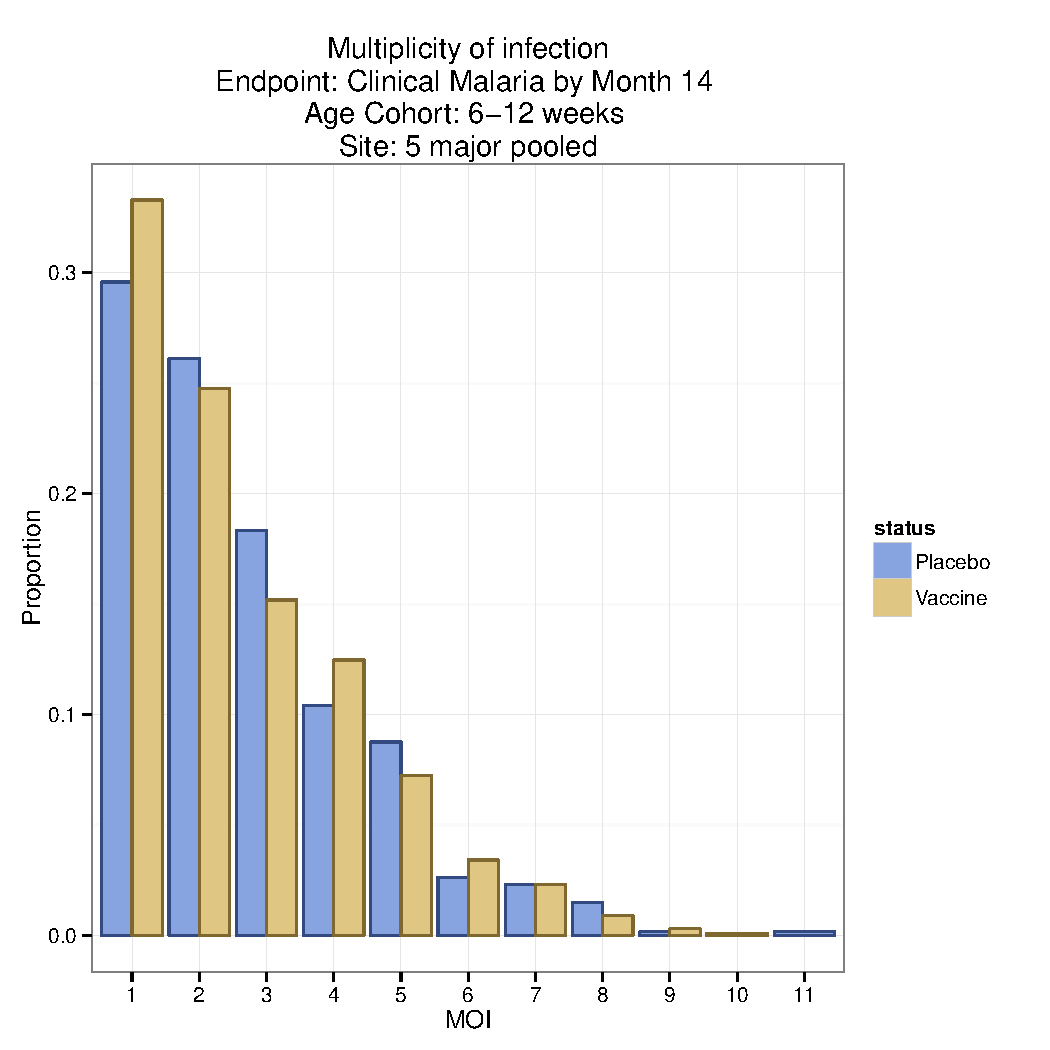
\includegraphics{figures/moi-newborn-c-1.pdf}
\caption{Descriptive plot of multiplicity}
\end{figure}

\begin{figure}[htbp]
\centering
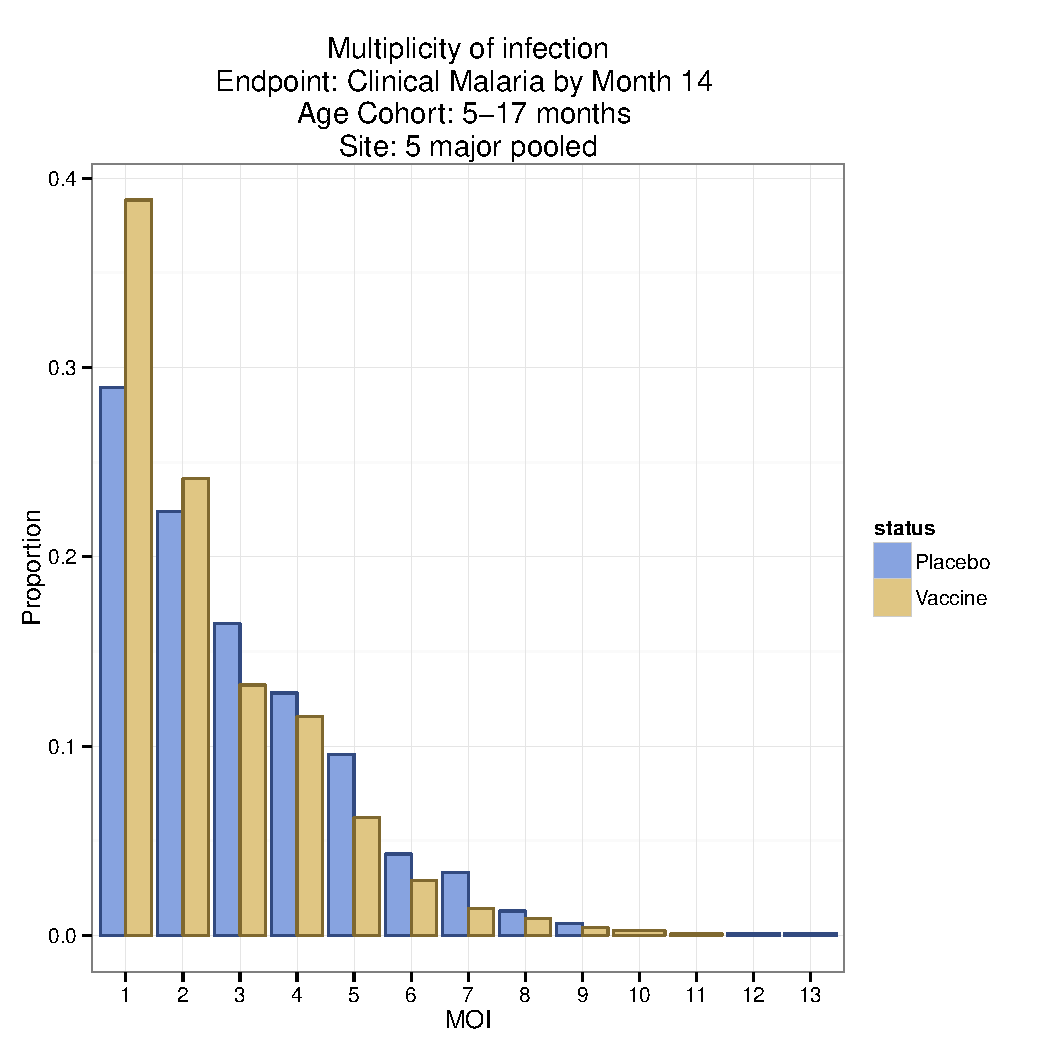
\includegraphics{figures/moi-infant-c-1.pdf}
\caption{Descriptive plot of multiplicity}
\end{figure}

\begin{figure}[htbp]
\centering
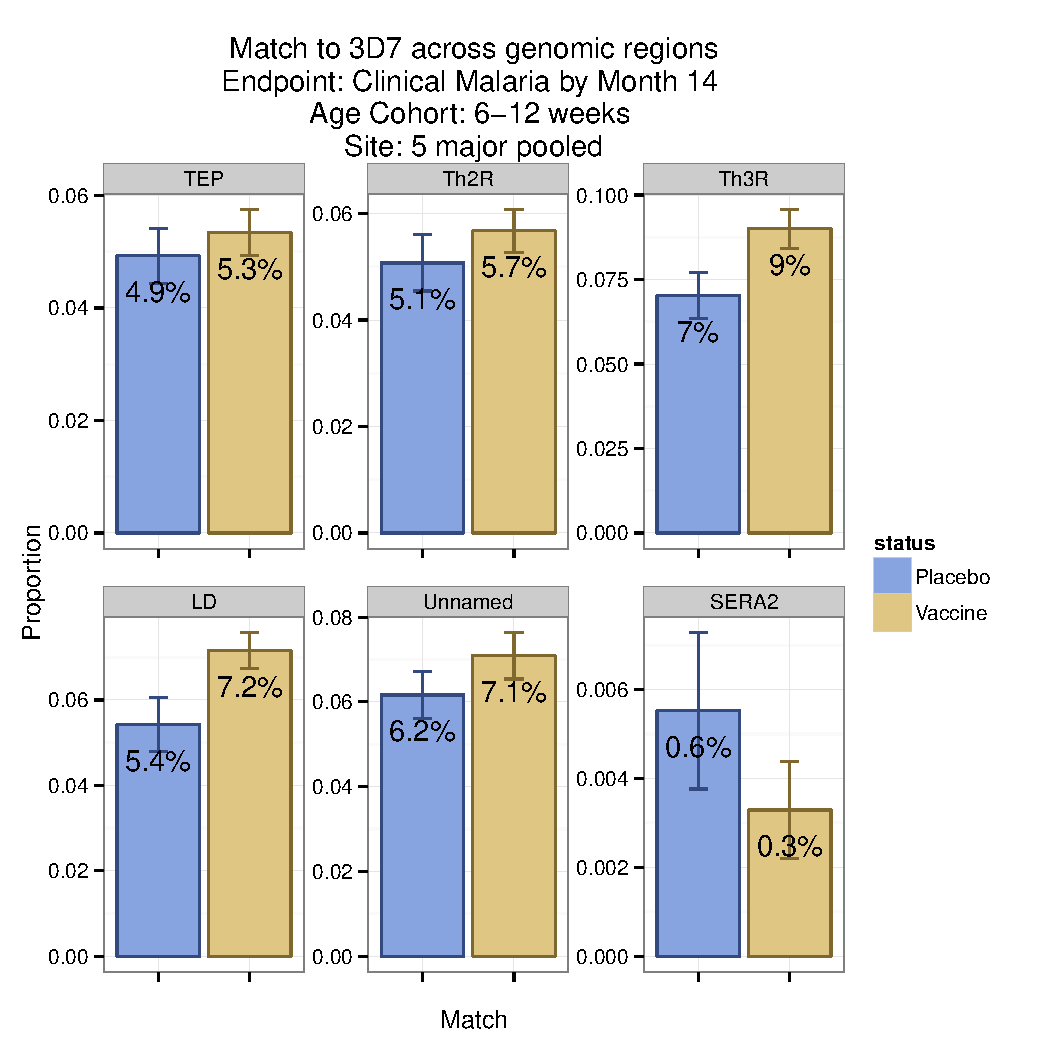
\includegraphics{figures/match-newborn-c-1.pdf}
\caption{Descriptive plot of match to 3D7 in C-terminus CSP}
\end{figure}

\begin{figure}[htbp]
\centering
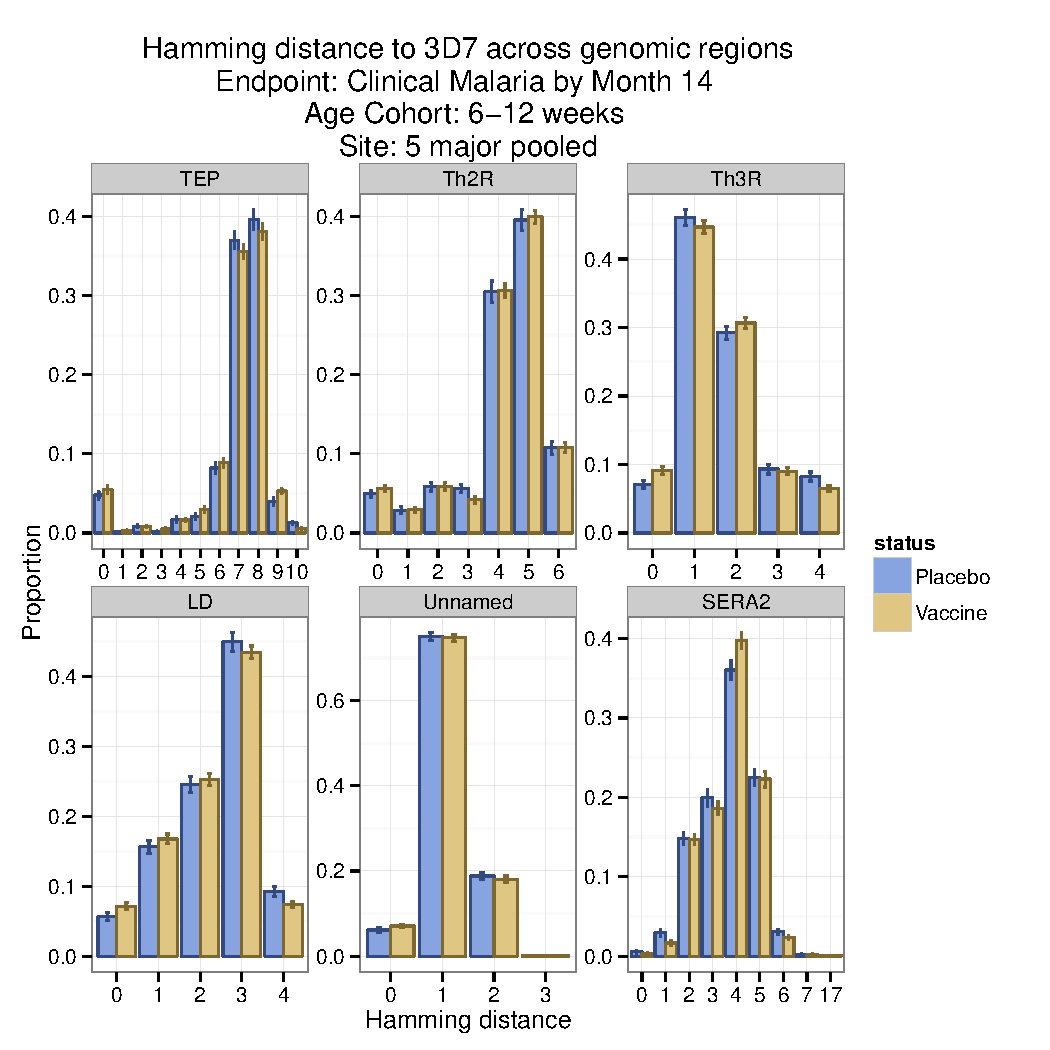
\includegraphics{figures/hamming-newborn-c-1.pdf}
\caption{Descriptive plot of Hamming distance to 3D7 in C-terminus CSP}
\end{figure}

\begin{figure}[htbp]
\centering
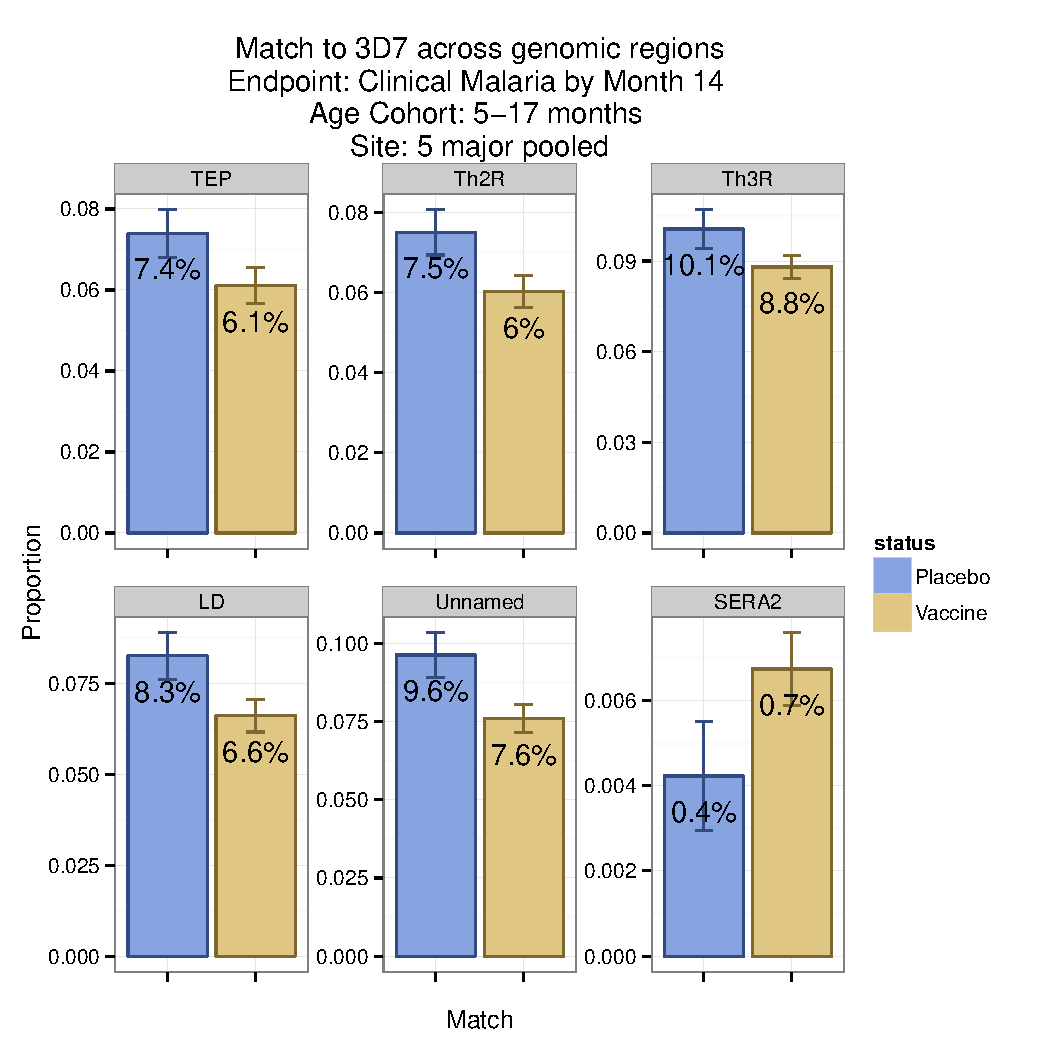
\includegraphics{figures/match-infant-c-1.pdf}
\caption{Descriptive plot of match to 3D7 in C-terminus CSP}
\end{figure}

\begin{figure}[htbp]
\centering
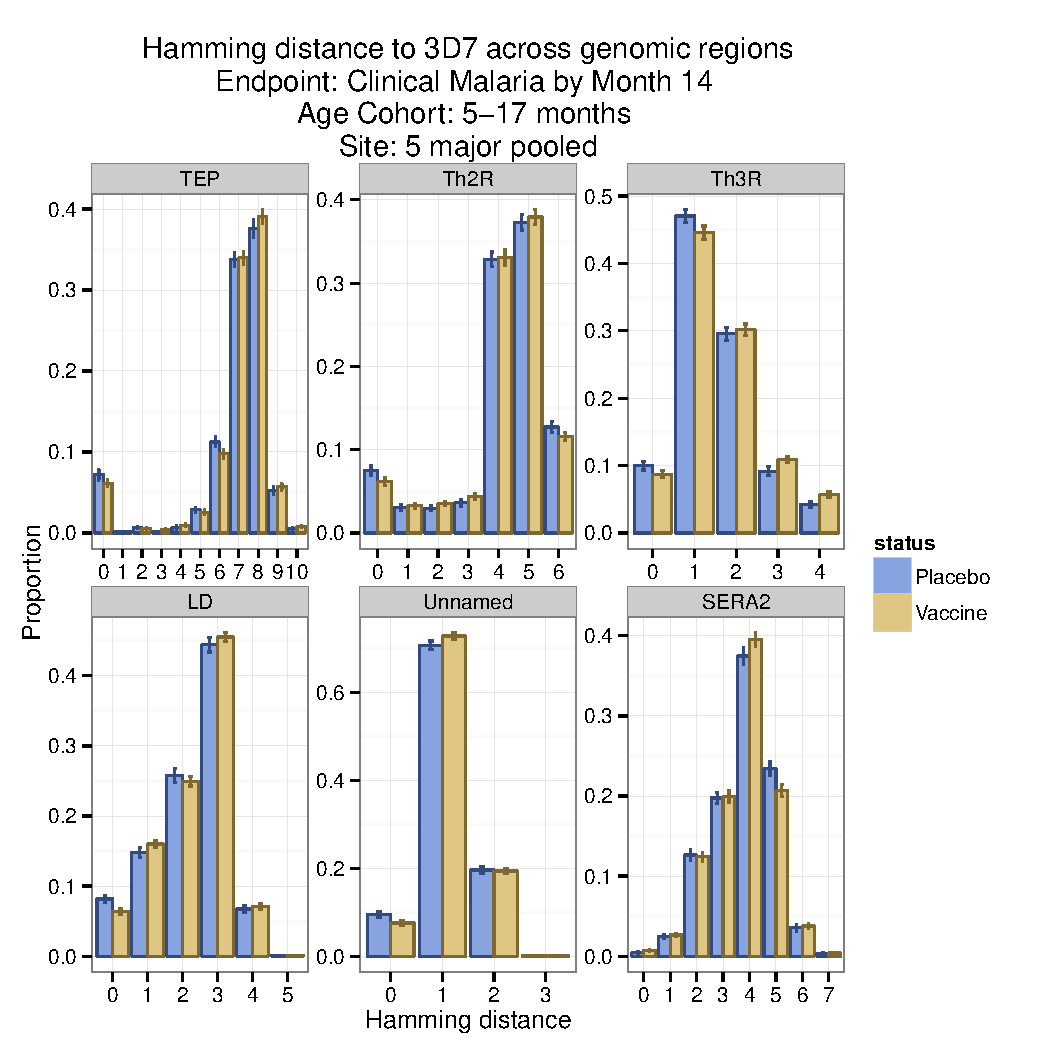
\includegraphics{figures/hamming-infant-c-1.pdf}
\caption{Descriptive plot of Hamming distance to 3D7 in C-terminus CSP}
\end{figure}

\begin{figure}[htbp]
\centering
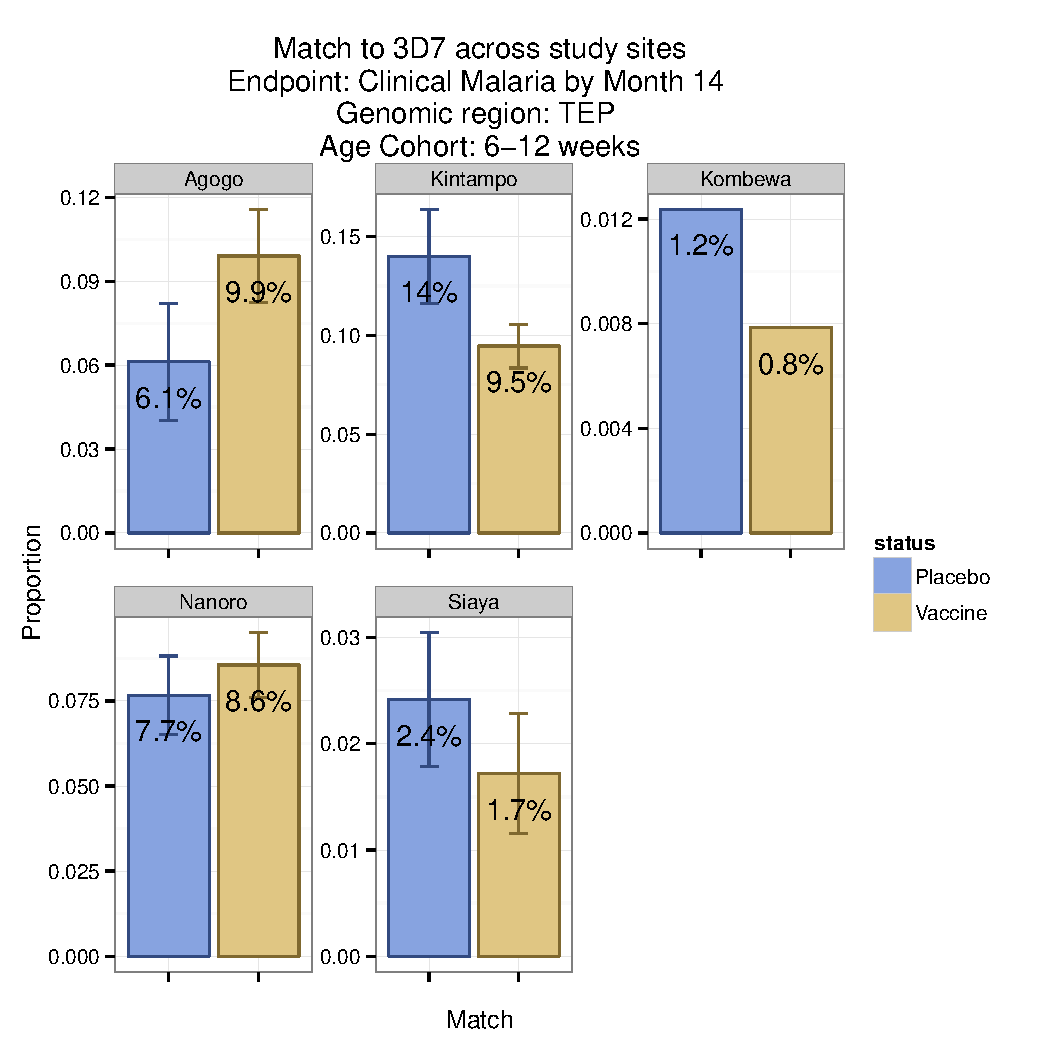
\includegraphics{figures/match-newborn-sites-c-1.pdf}
\caption{Descriptive plot of match to 3D7 in C-terminus CSP}
\end{figure}

\begin{figure}[htbp]
\centering
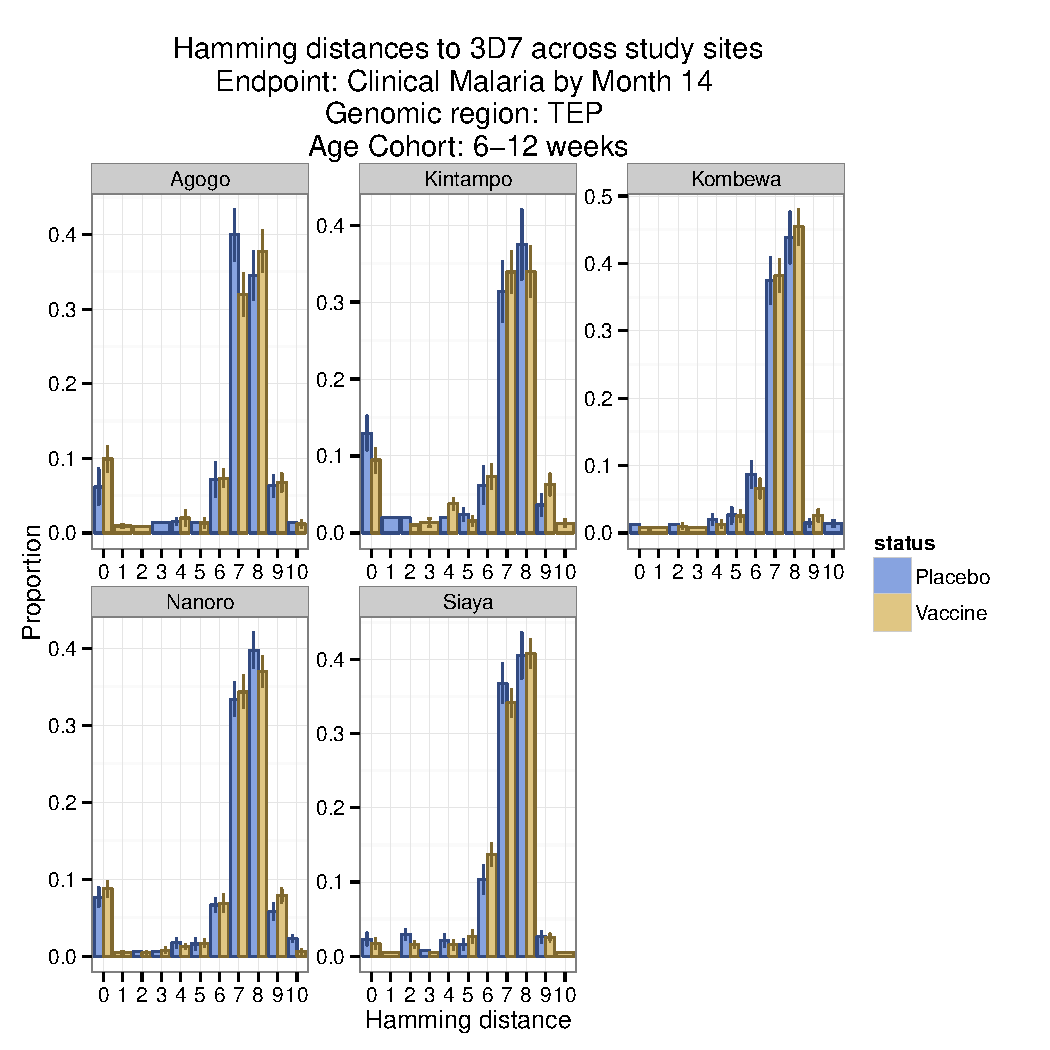
\includegraphics{figures/hamming-newborn-sites-c-1.pdf}
\caption{Descriptive plot of Hamming distance to 3D7 in C-terminus CSP}
\end{figure}

\begin{figure}[htbp]
\centering
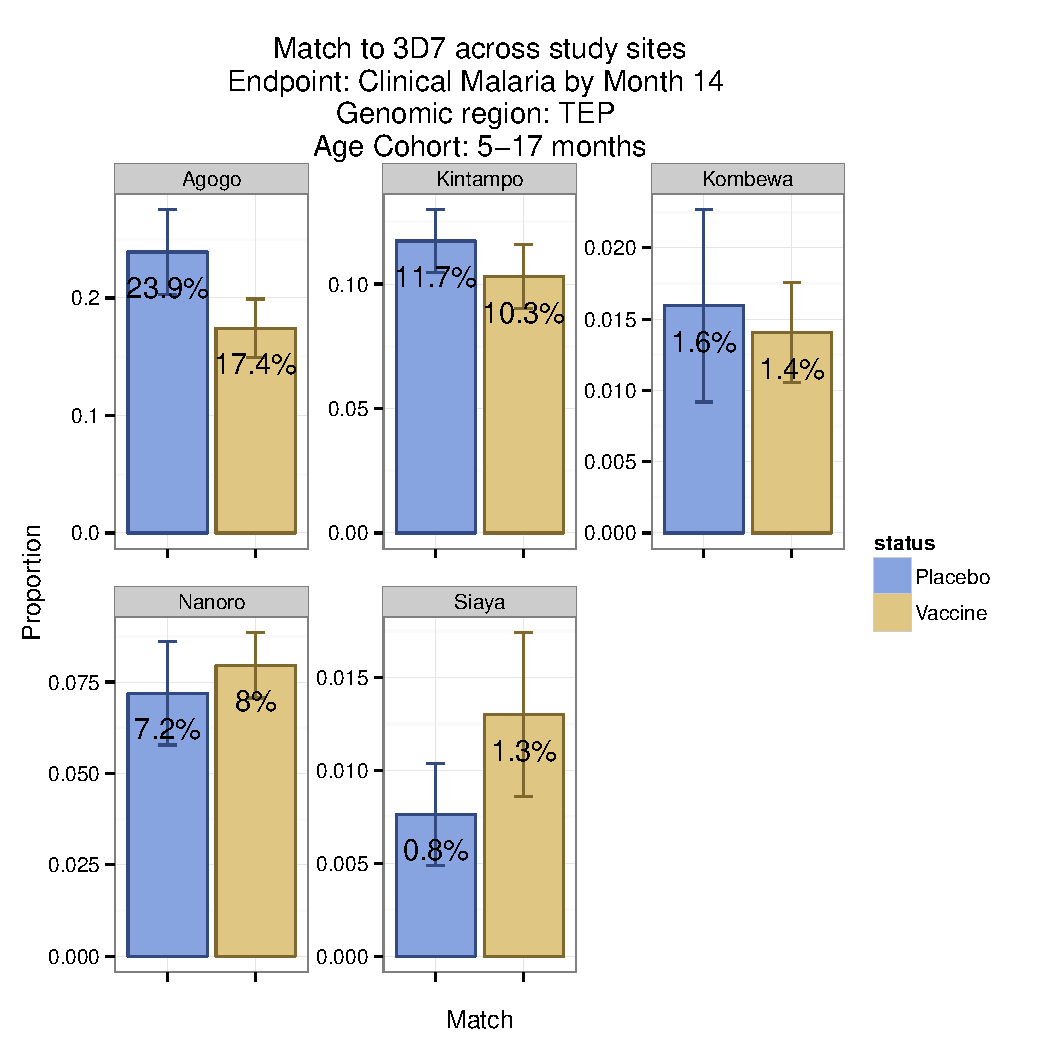
\includegraphics{figures/match-infant-sites-c-1.pdf}
\caption{Descriptive plot of match to 3D7 in C-terminus CSP}
\end{figure}

\begin{figure}[htbp]
\centering
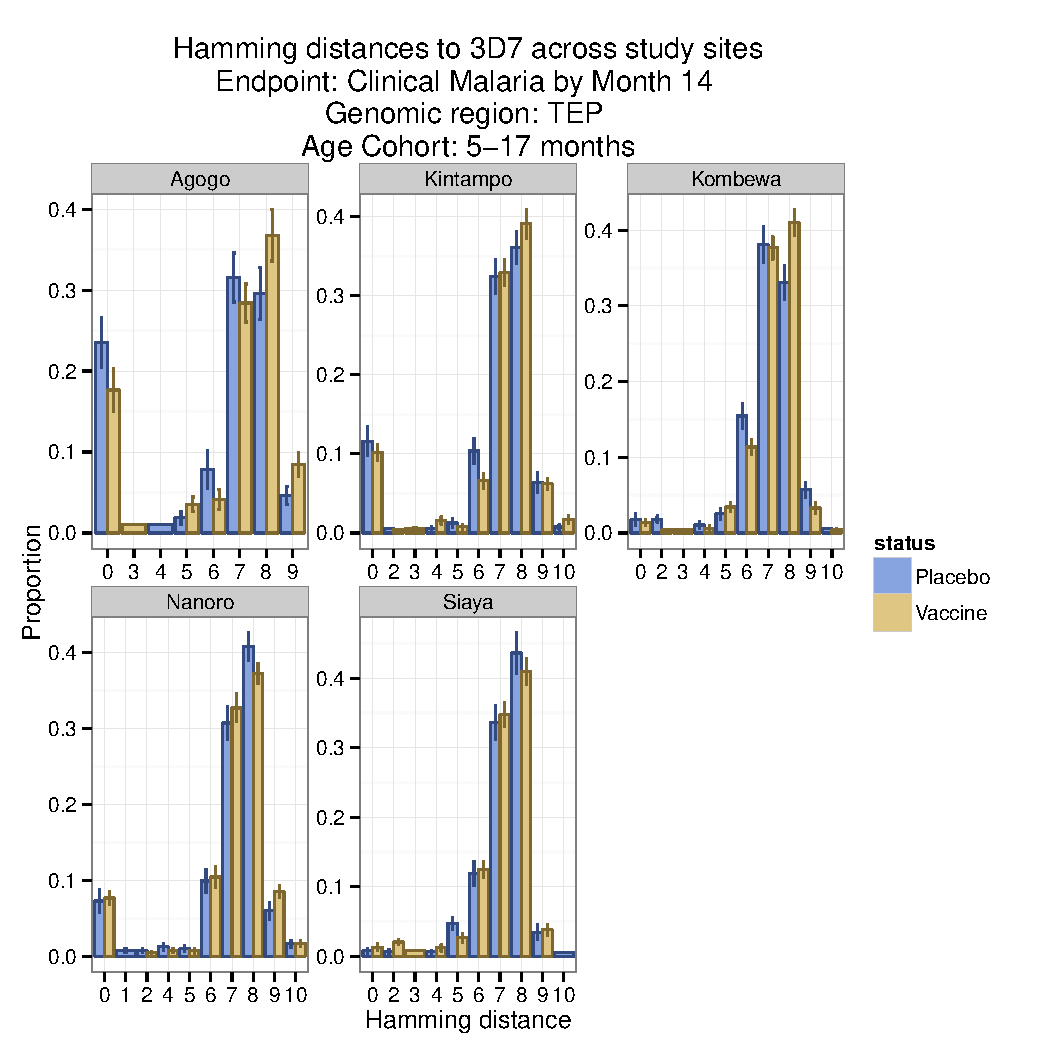
\includegraphics{figures/hamming-infant-sites-c-1.pdf}
\caption{Descriptive plot of Hamming distance to 3D7 in C-terminus CSP}
\end{figure}

\begin{figure}[htbp]
\centering
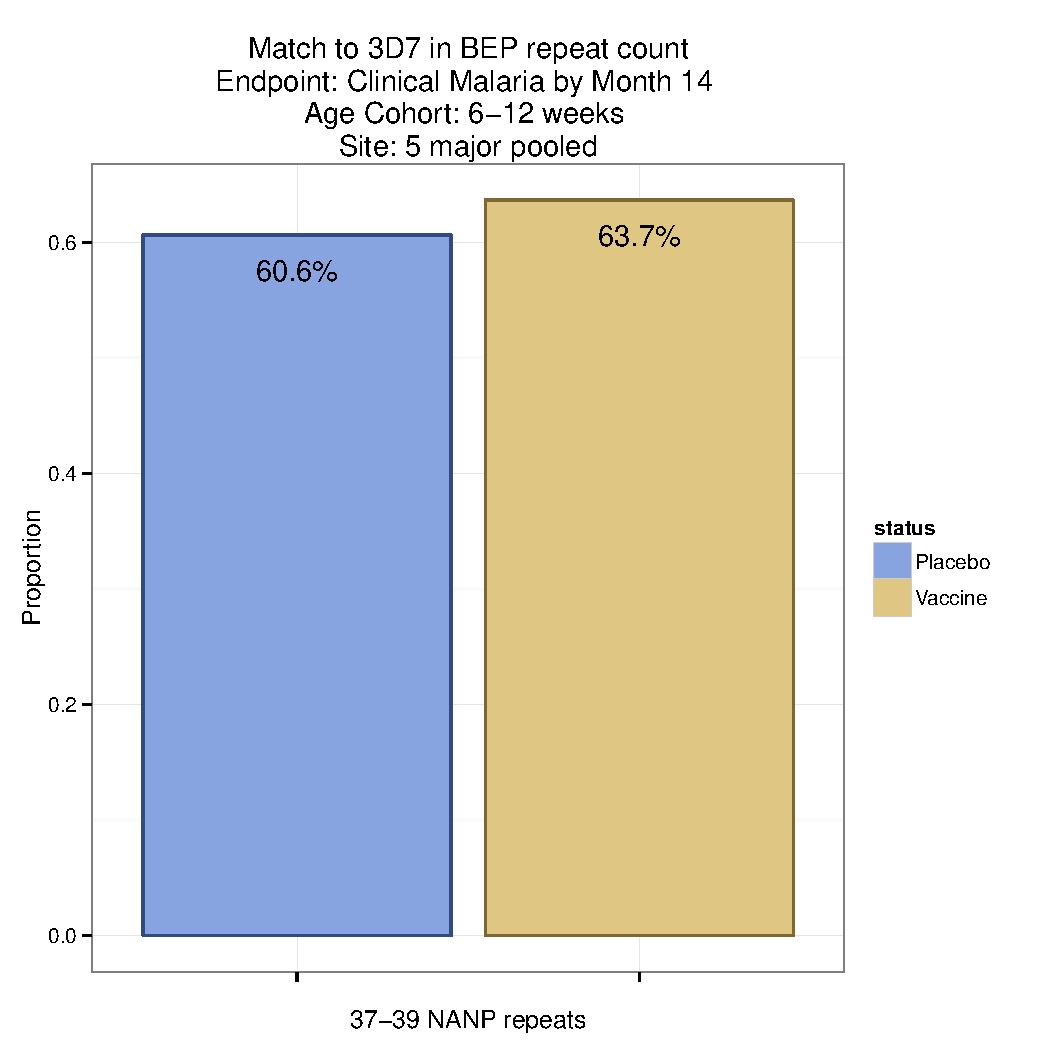
\includegraphics{figures/bep-match-newborn-c-1.pdf}
\caption{Descriptive plot of match to 3D7 in NANP repeat region}
\end{figure}

\begin{figure}[htbp]
\centering
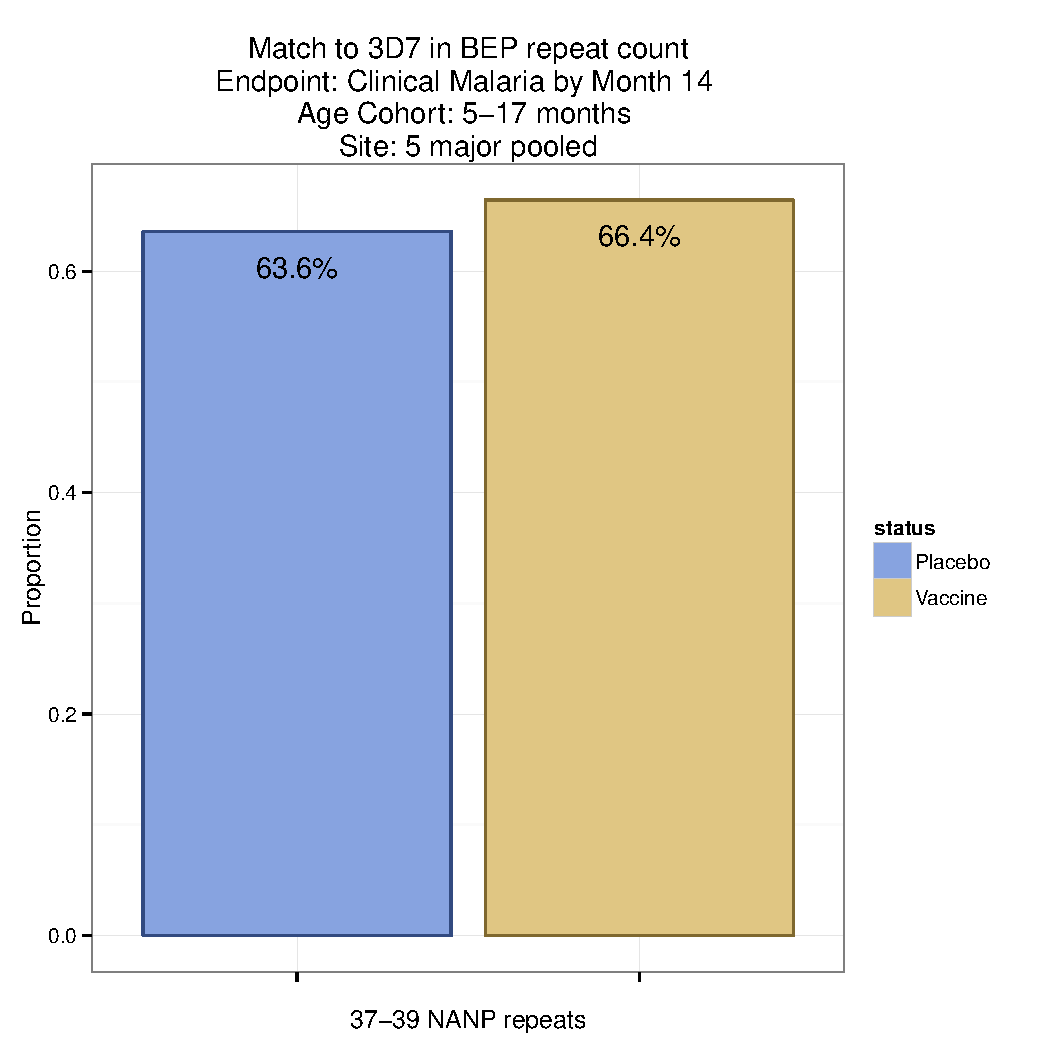
\includegraphics{figures/bep-match-infact-c-1.pdf}
\caption{Descriptive plot of match to 3D7 in NANP repeat region}
\end{figure}

\begin{figure}[htbp]
\centering
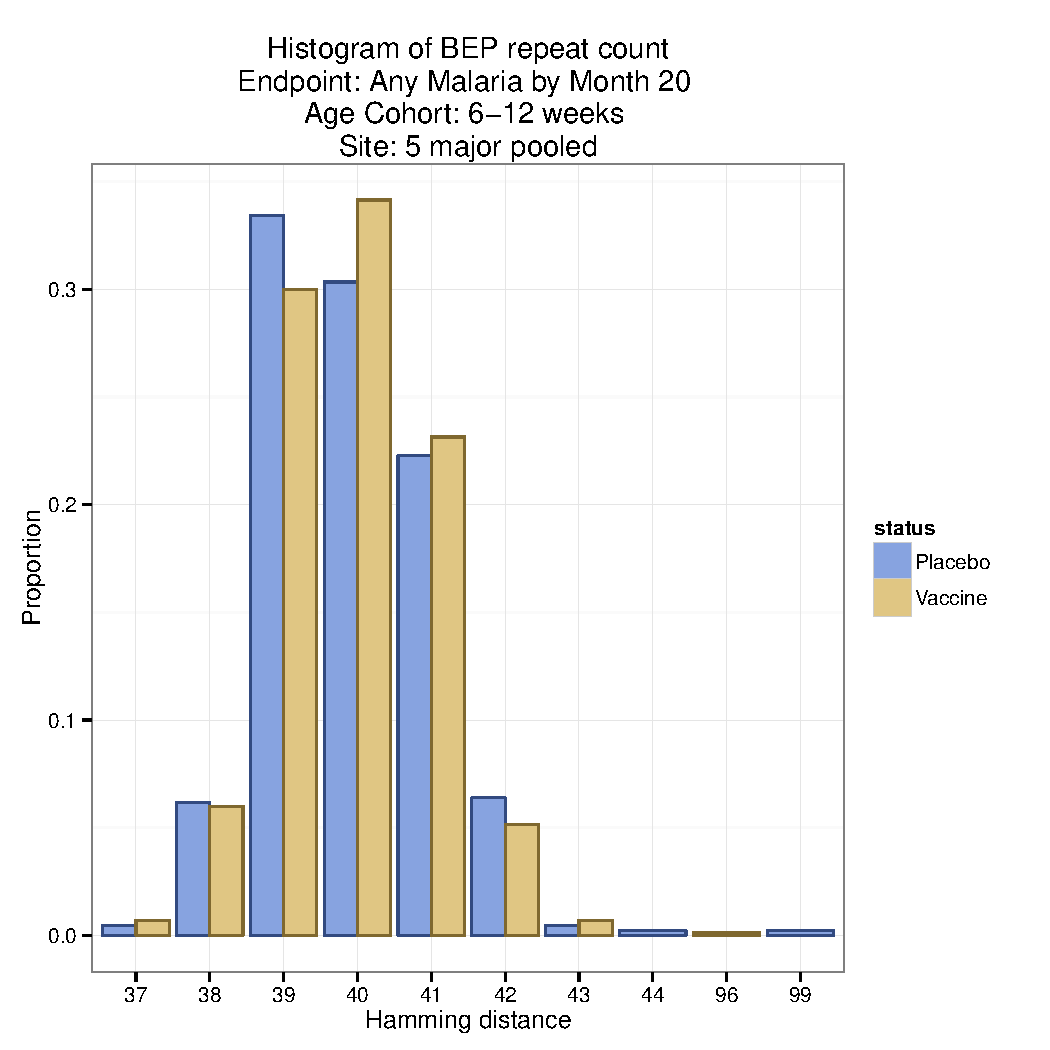
\includegraphics{figures/bep-hist-newborn-c-1.pdf}
\caption{Descriptive plot of NANP repeat distribution}
\end{figure}

\begin{figure}[htbp]
\centering
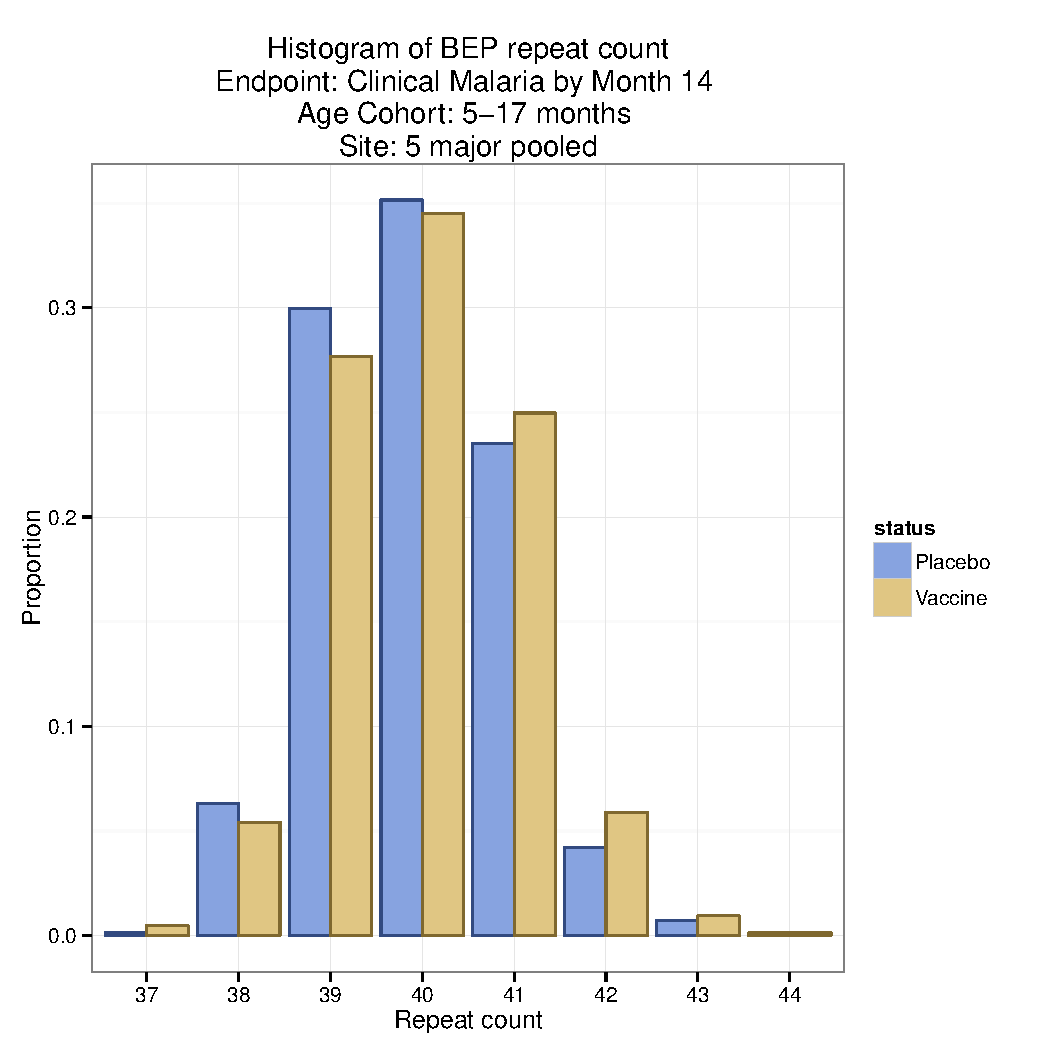
\includegraphics{figures/bep-hist-infant-c-1.pdf}
\caption{Descriptive plot of NANP repeat distribution}
\end{figure}

\begin{figure}[htbp]
\centering
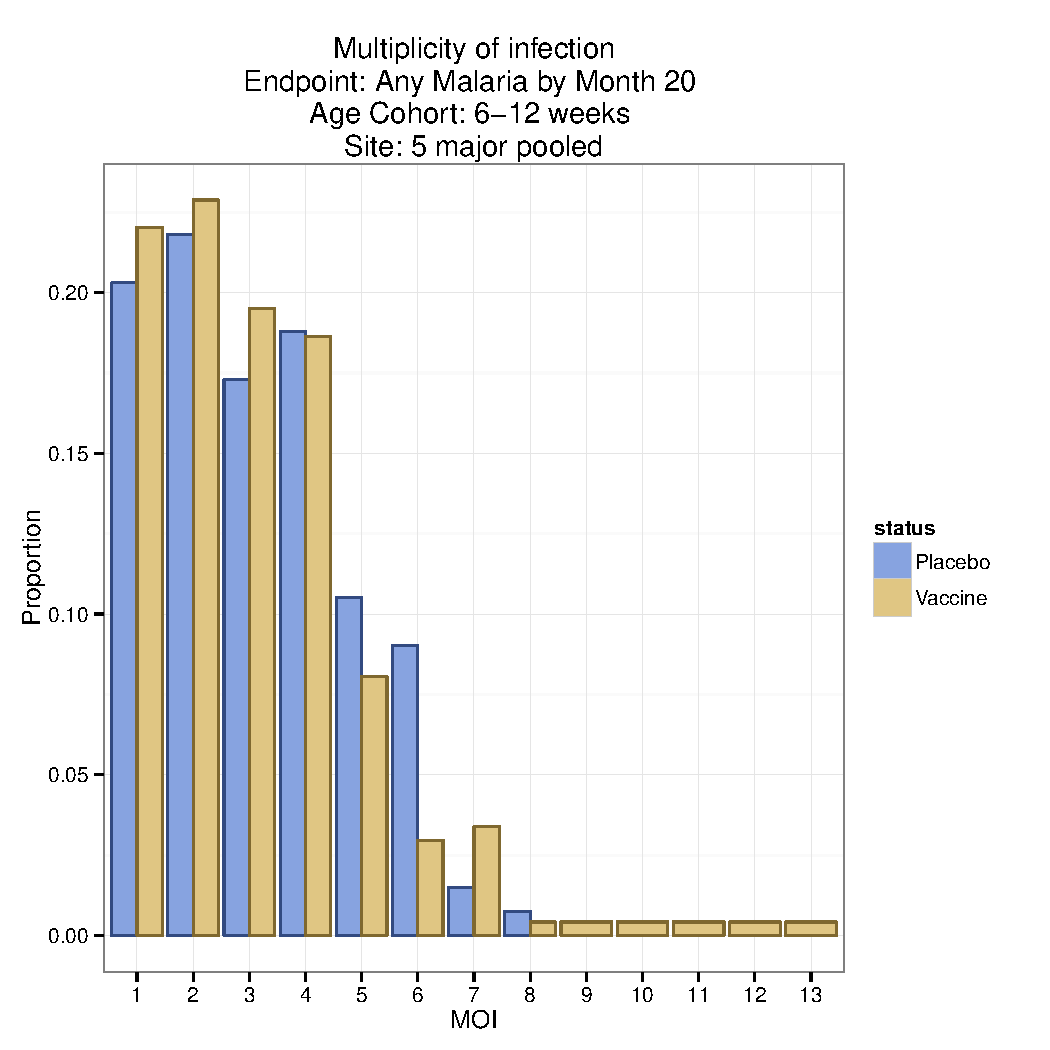
\includegraphics{figures/moi-newborn-x-1.pdf}
\caption{Descriptive plot of multiplicity}
\end{figure}

\begin{figure}[htbp]
\centering
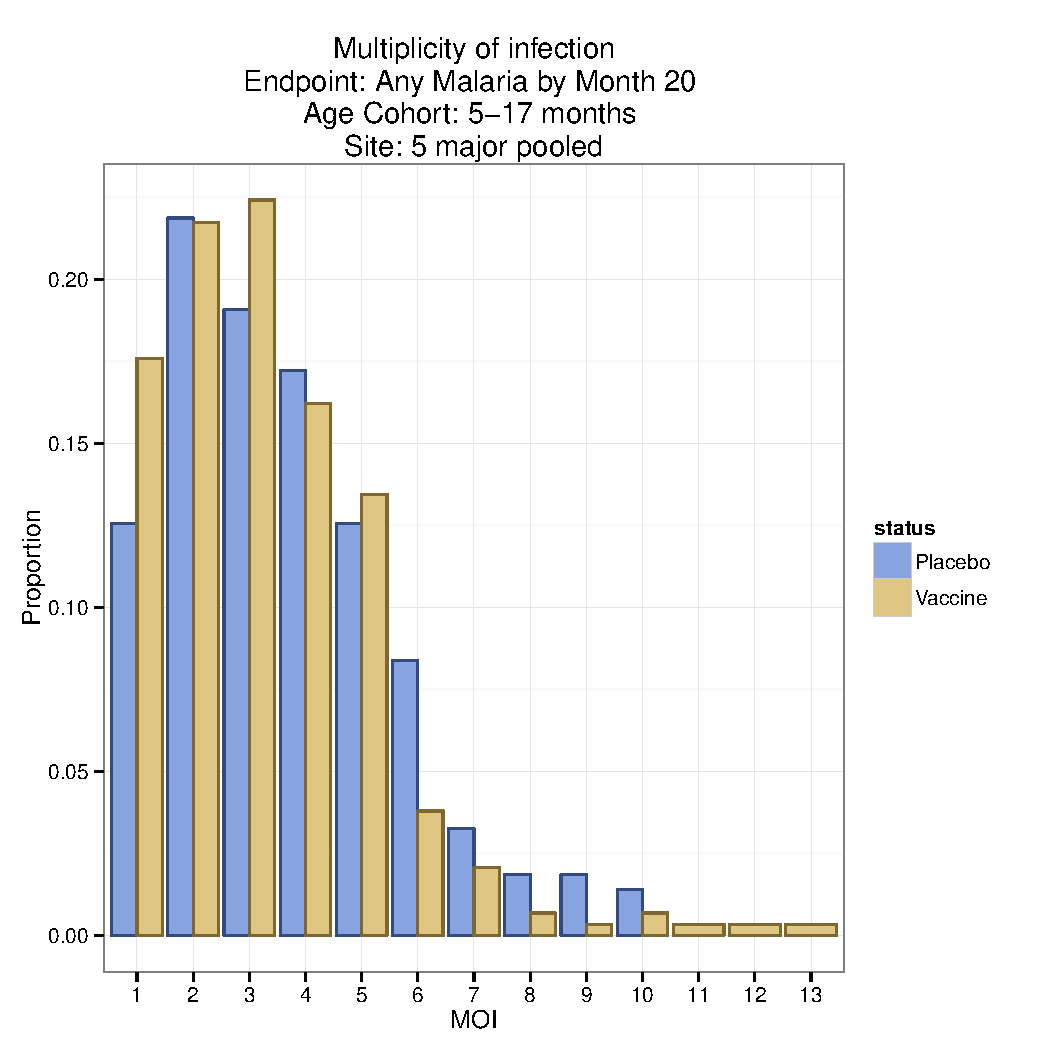
\includegraphics{figures/moi-infant-x-1.pdf}
\caption{Descriptive plot of multiplicity}
\end{figure}

\begin{figure}[htbp]
\centering
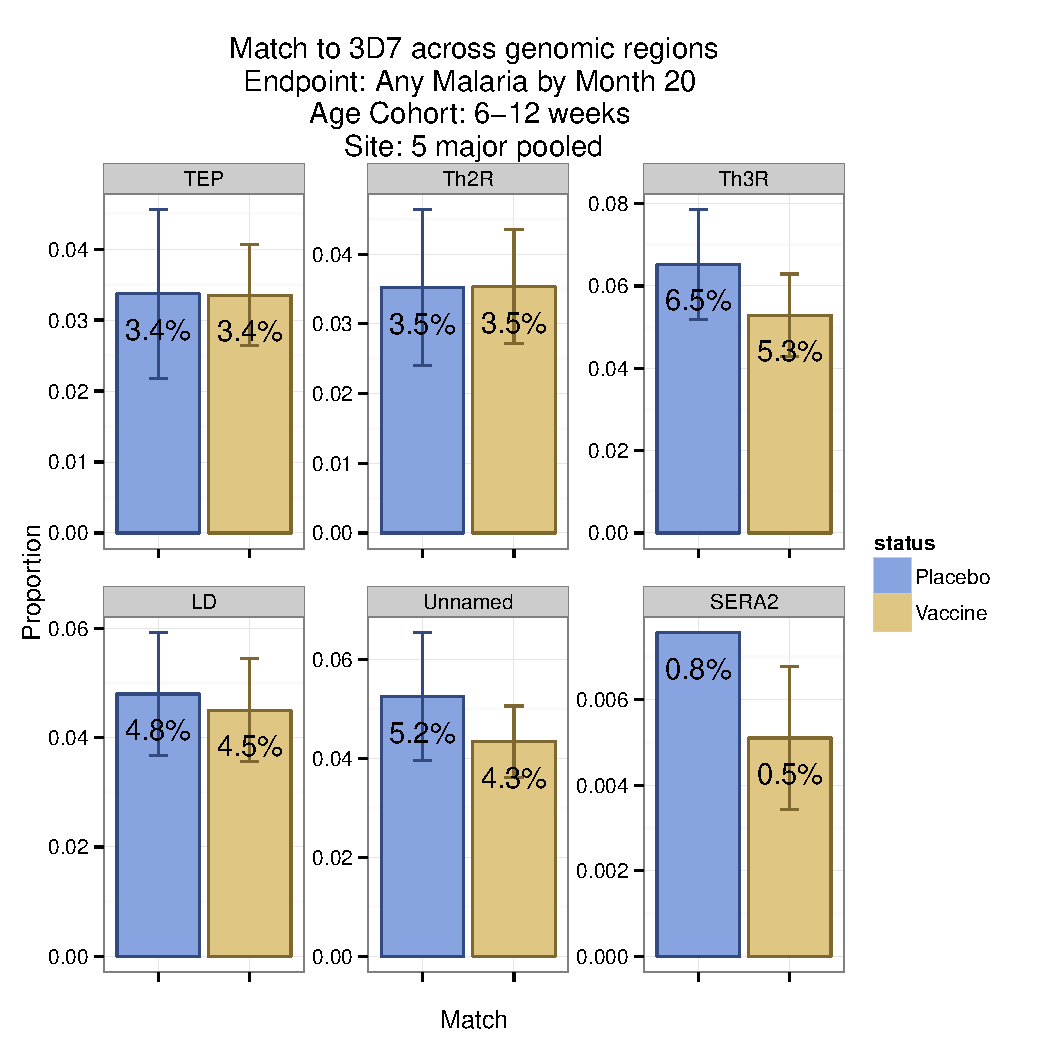
\includegraphics{figures/match-newborn-x-1.pdf}
\caption{Descriptive plot of match to 3D7 in C-terminus CSP}
\end{figure}

\begin{figure}[htbp]
\centering
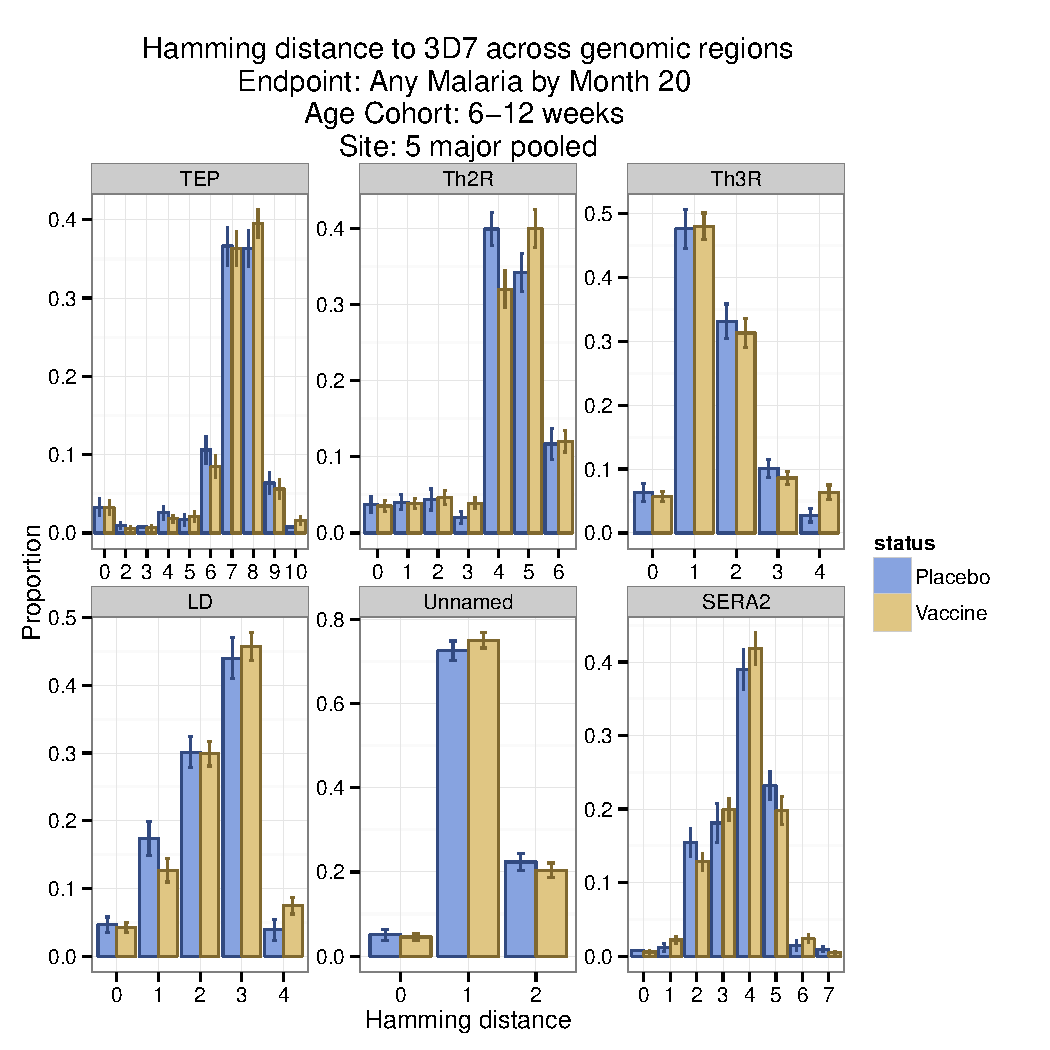
\includegraphics{figures/hamming-newborn-x-1.pdf}
\caption{Descriptive plot of Hamming distance to 3D7 in C-terminus CSP}
\end{figure}

\begin{figure}[htbp]
\centering
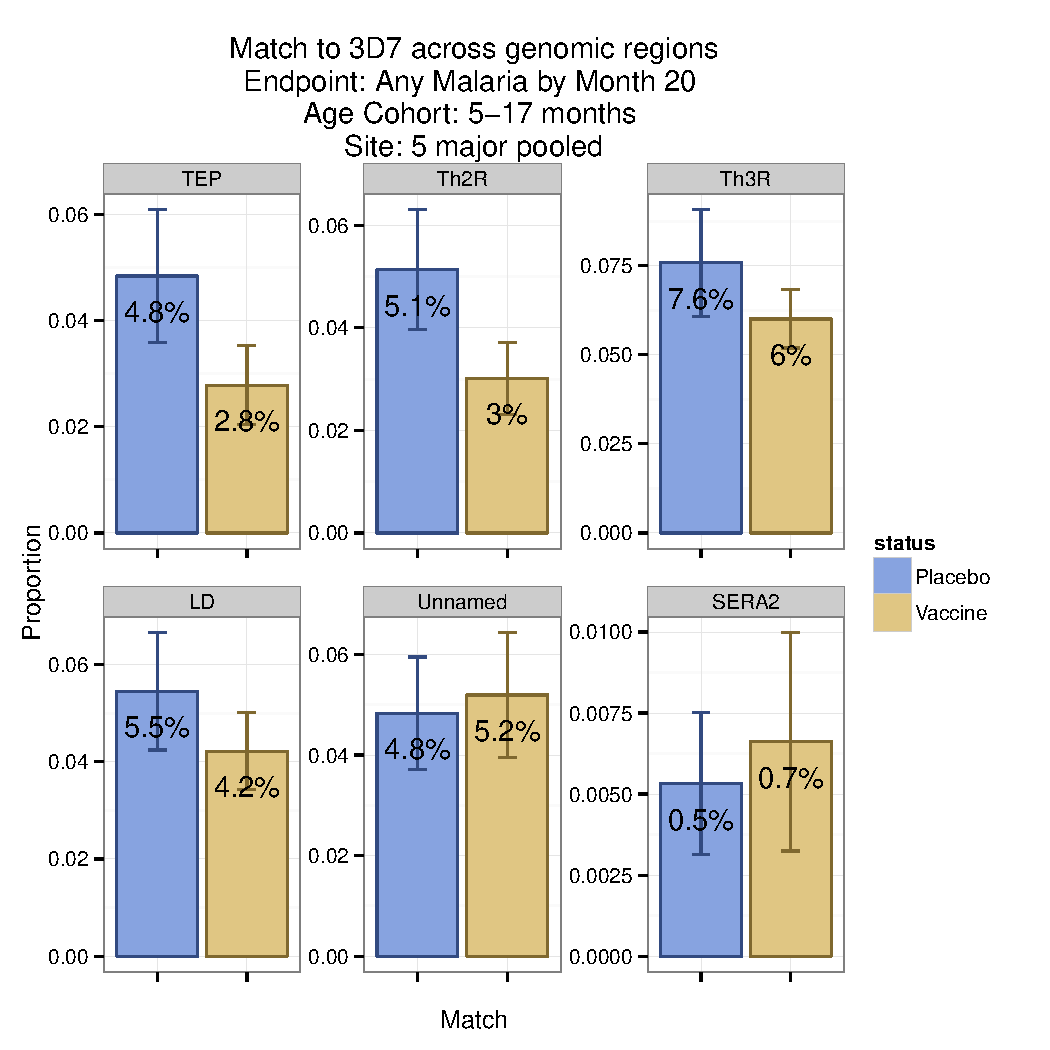
\includegraphics{figures/match-infant-x-1.pdf}
\caption{Descriptive plot of match to 3D7 in C-terminus CSP}
\end{figure}

\begin{figure}[htbp]
\centering
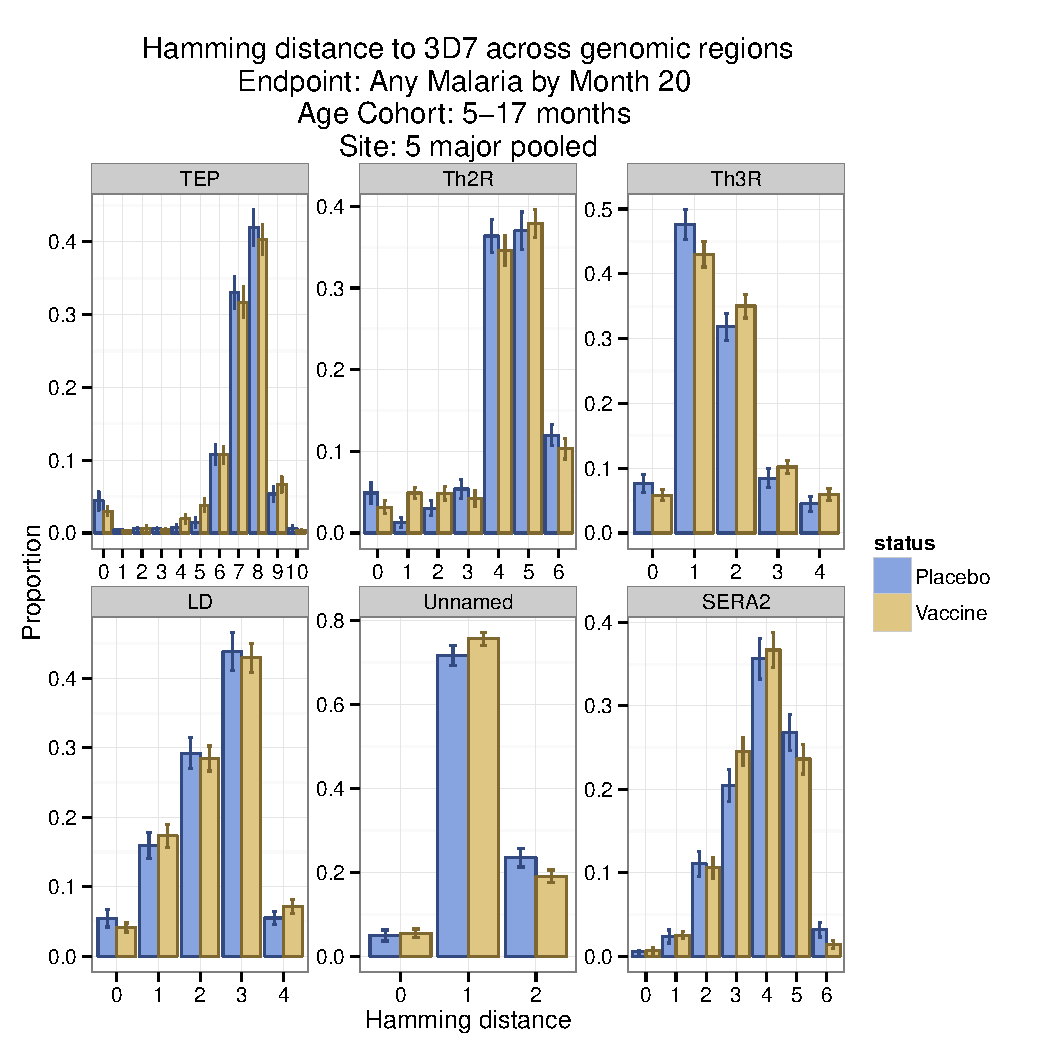
\includegraphics{figures/hamming-infant-x-1.pdf}
\caption{Descriptive plot of Hamming distance to 3D7 in C-terminus CSP}
\end{figure}

\begin{figure}[htbp]
\centering
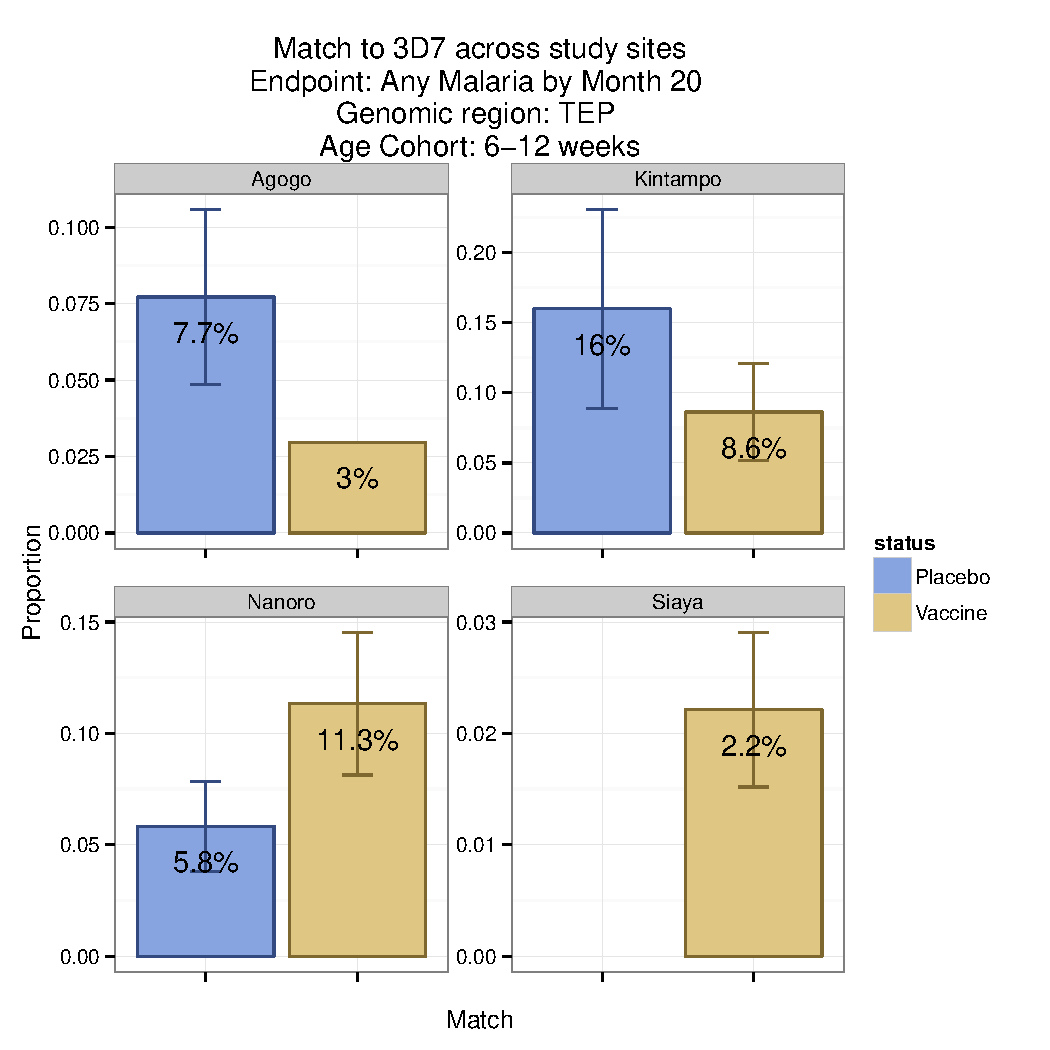
\includegraphics{figures/match-newborn-sites-x-1.pdf}
\caption{Descriptive plot of match to 3D7 in C-terminus CSP}
\end{figure}

\begin{figure}[htbp]
\centering
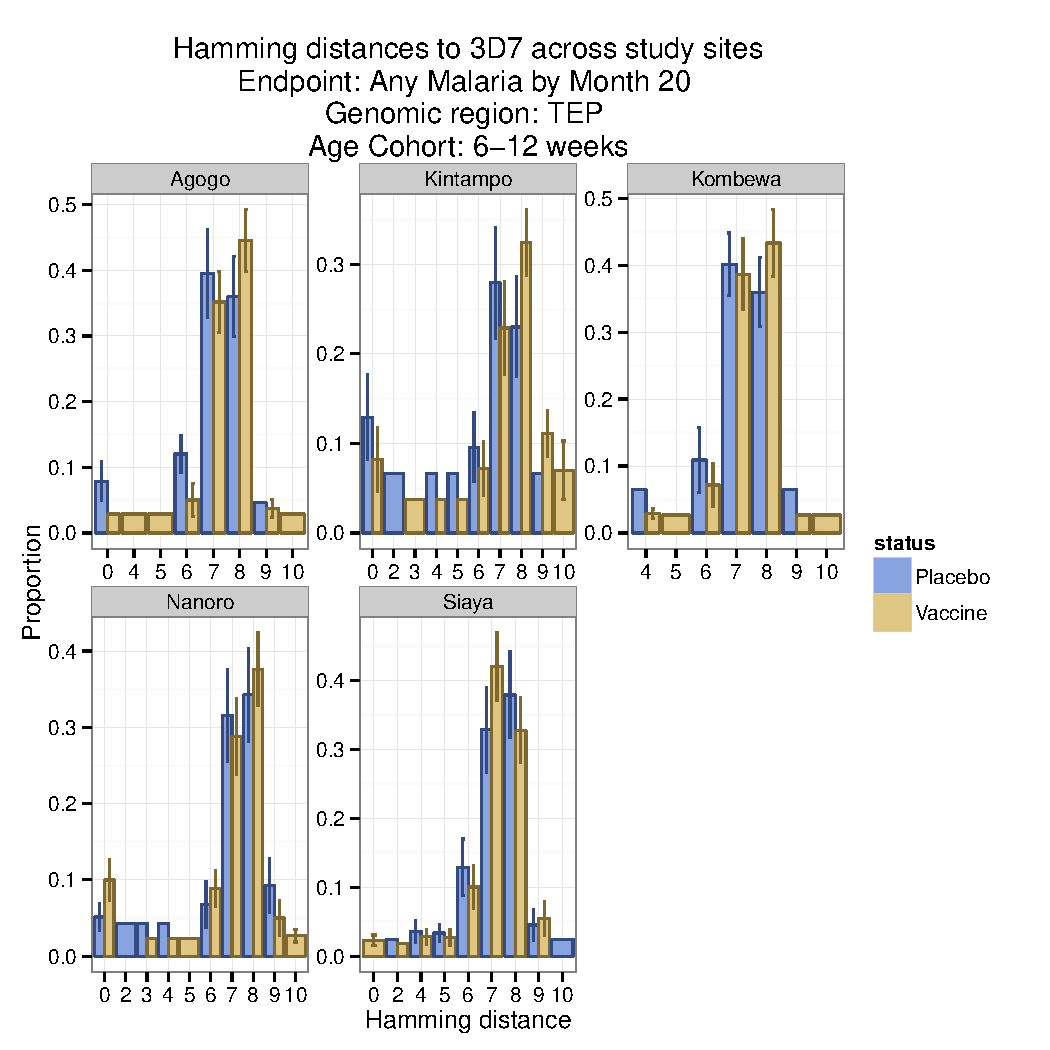
\includegraphics{figures/hamming-newborn-sites-x-1.pdf}
\caption{Descriptive plot of Hamming distance to 3D7 in C-terminus CSP}
\end{figure}

\begin{figure}[htbp]
\centering
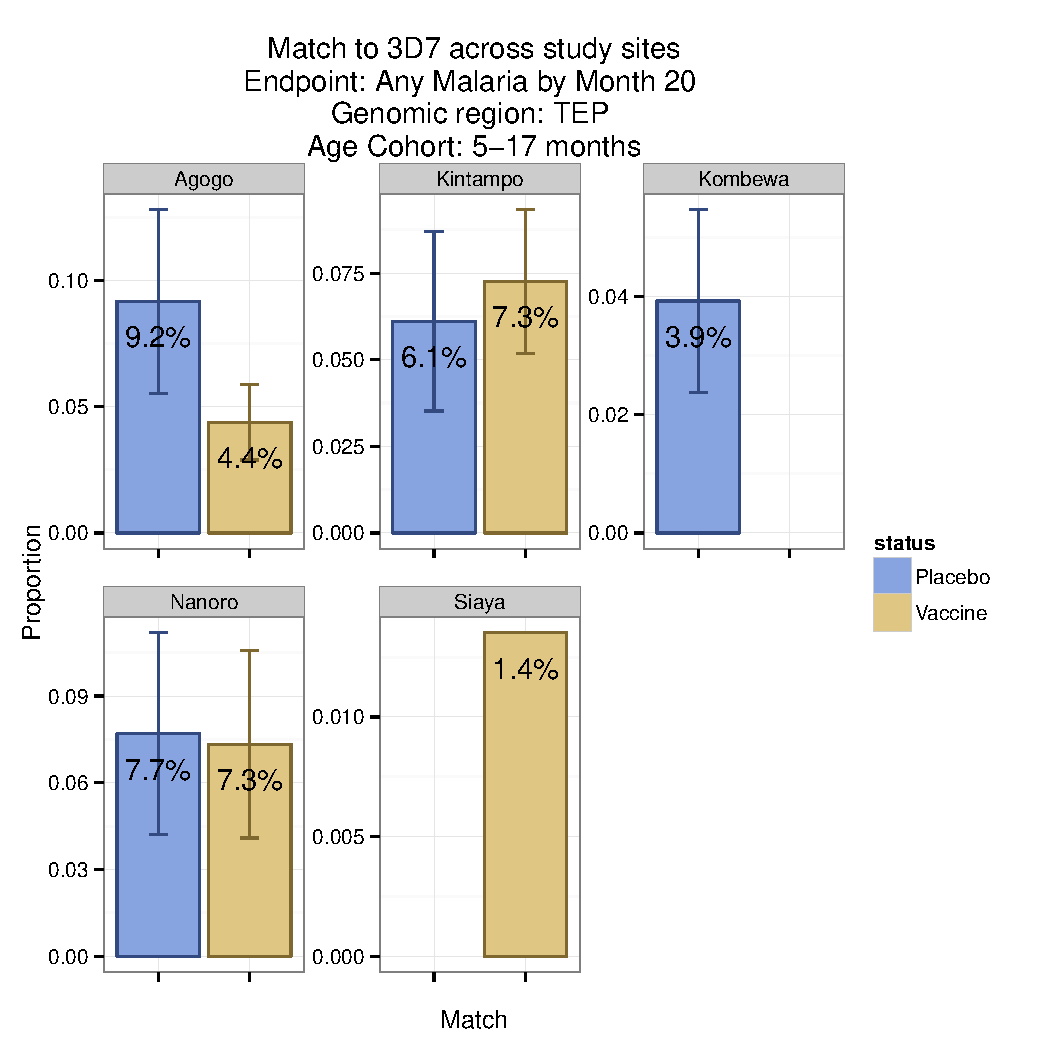
\includegraphics{figures/match-infant-sites-x-1.pdf}
\caption{Descriptive plot of match to 3D7 in C-terminus CSP}
\end{figure}

\begin{figure}[htbp]
\centering
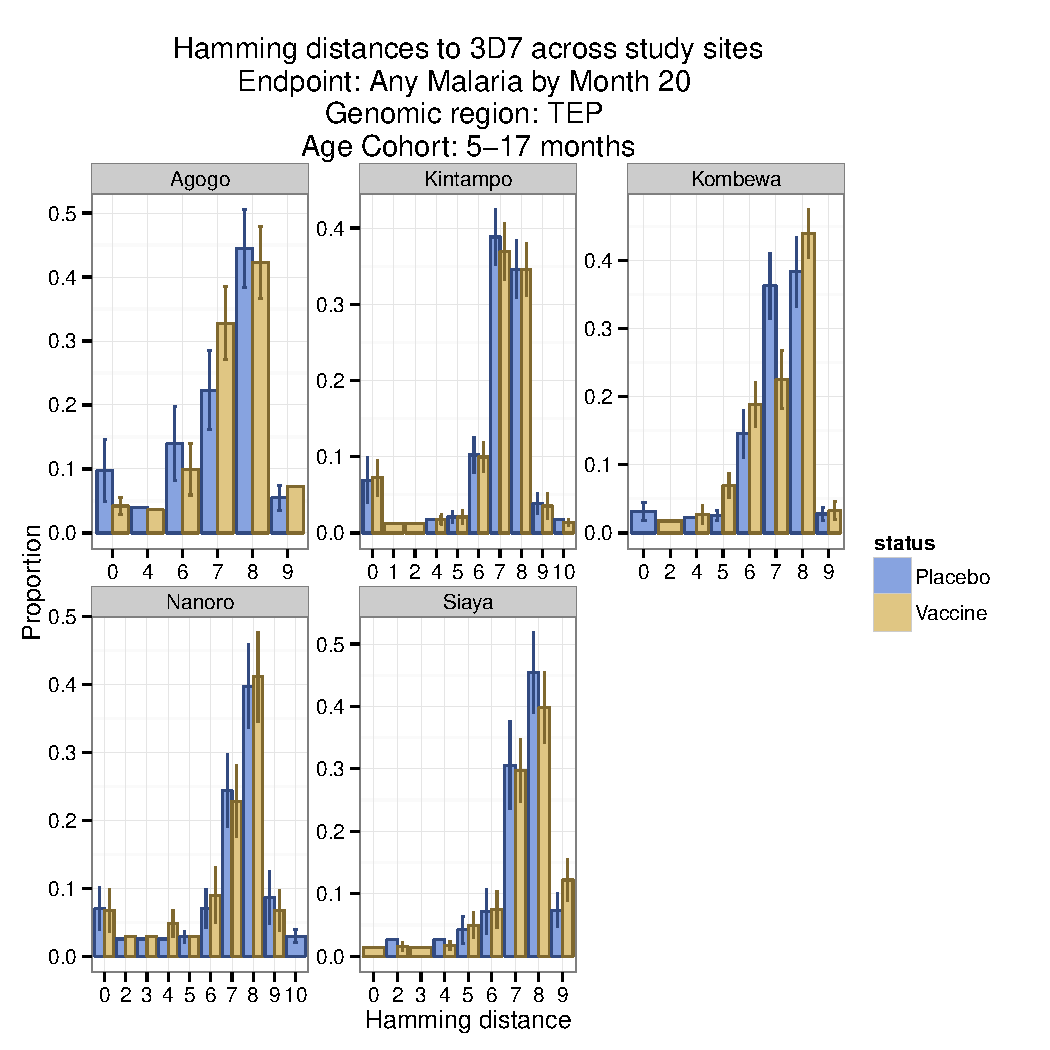
\includegraphics{figures/hamming-infant-sites-x-1.pdf}
\caption{Descriptive plot of Hamming distance to 3D7 in C-terminus CSP}
\end{figure}

\begin{figure}[htbp]
\centering
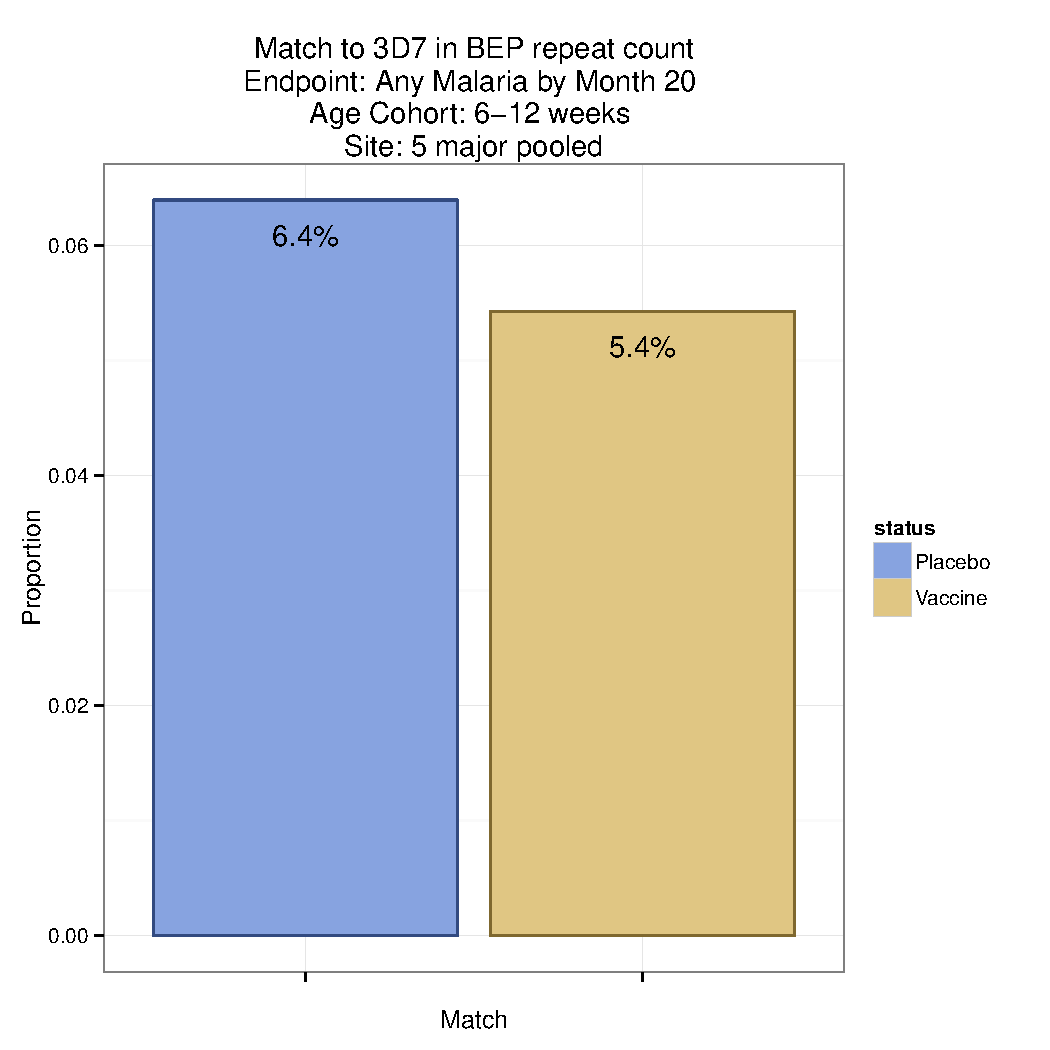
\includegraphics{figures/bep-match-newborn-x-1.pdf}
\caption{Descriptive plot of match to 3D7 in NANP repeat region}
\end{figure}

\begin{figure}[htbp]
\centering
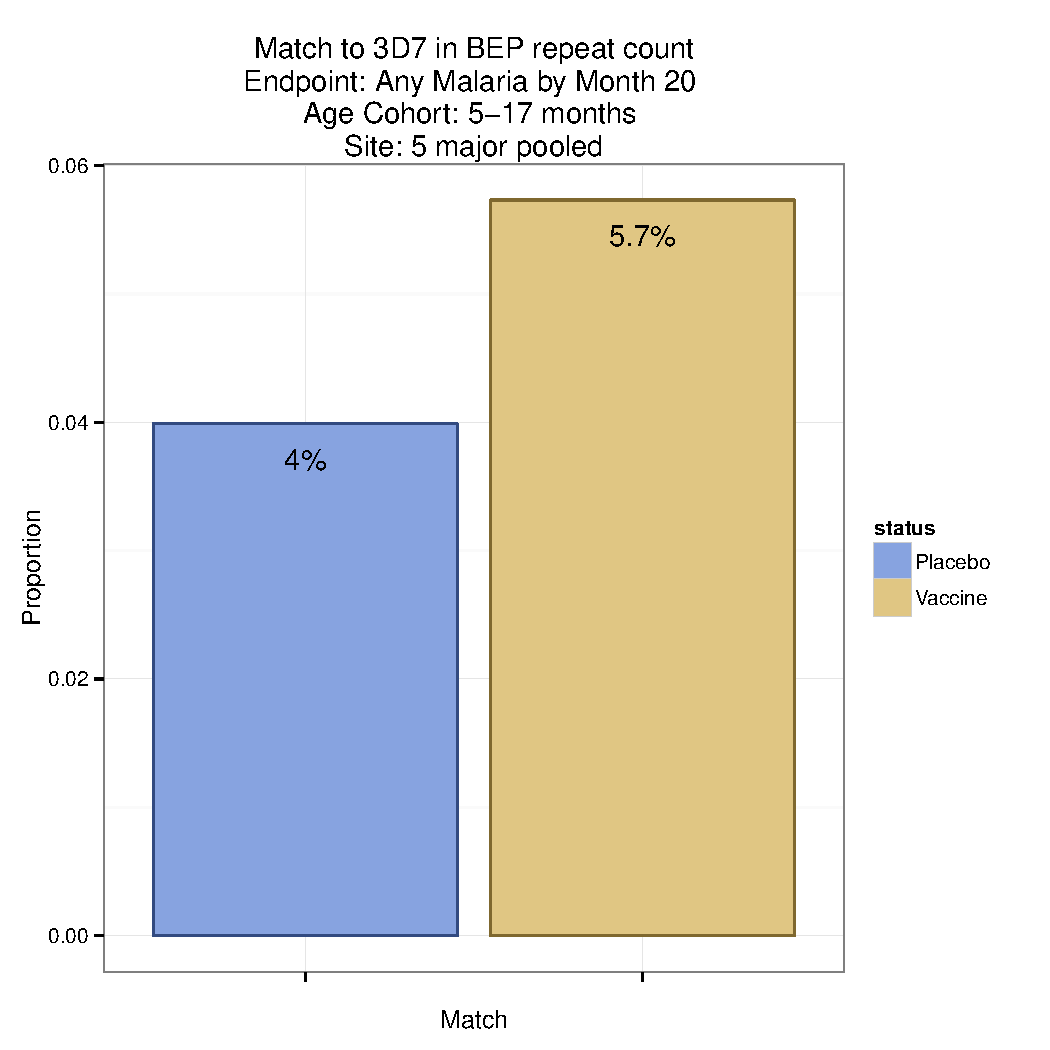
\includegraphics{figures/bep-match-infact-x-1.pdf}
\caption{Descriptive plot of match to 3D7 in NANP repeat region}
\end{figure}

\begin{figure}[htbp]
\centering
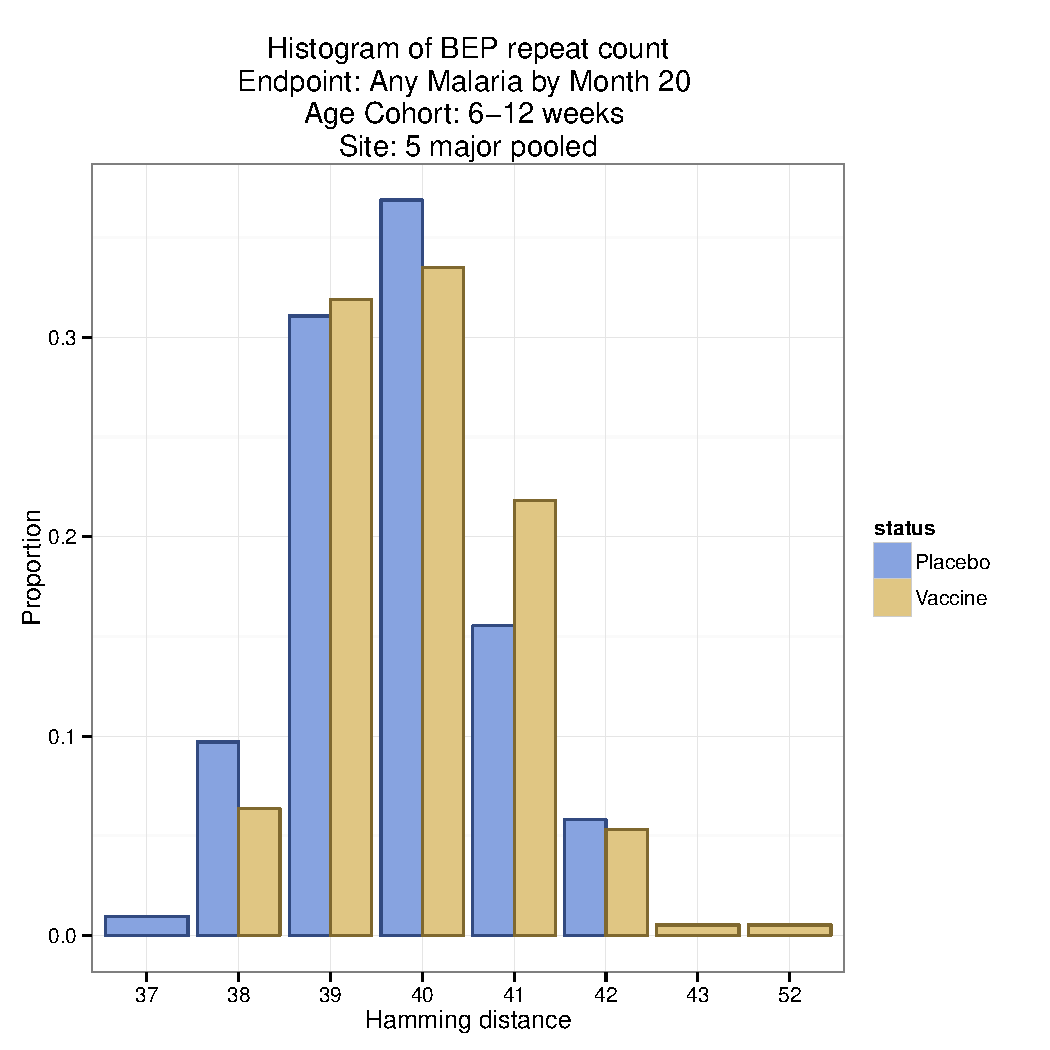
\includegraphics{figures/bep-hist-newborn-x-1.pdf}
\caption{Descriptive plot of NANP repeat distribution}
\end{figure}

\begin{figure}[htbp]
\centering
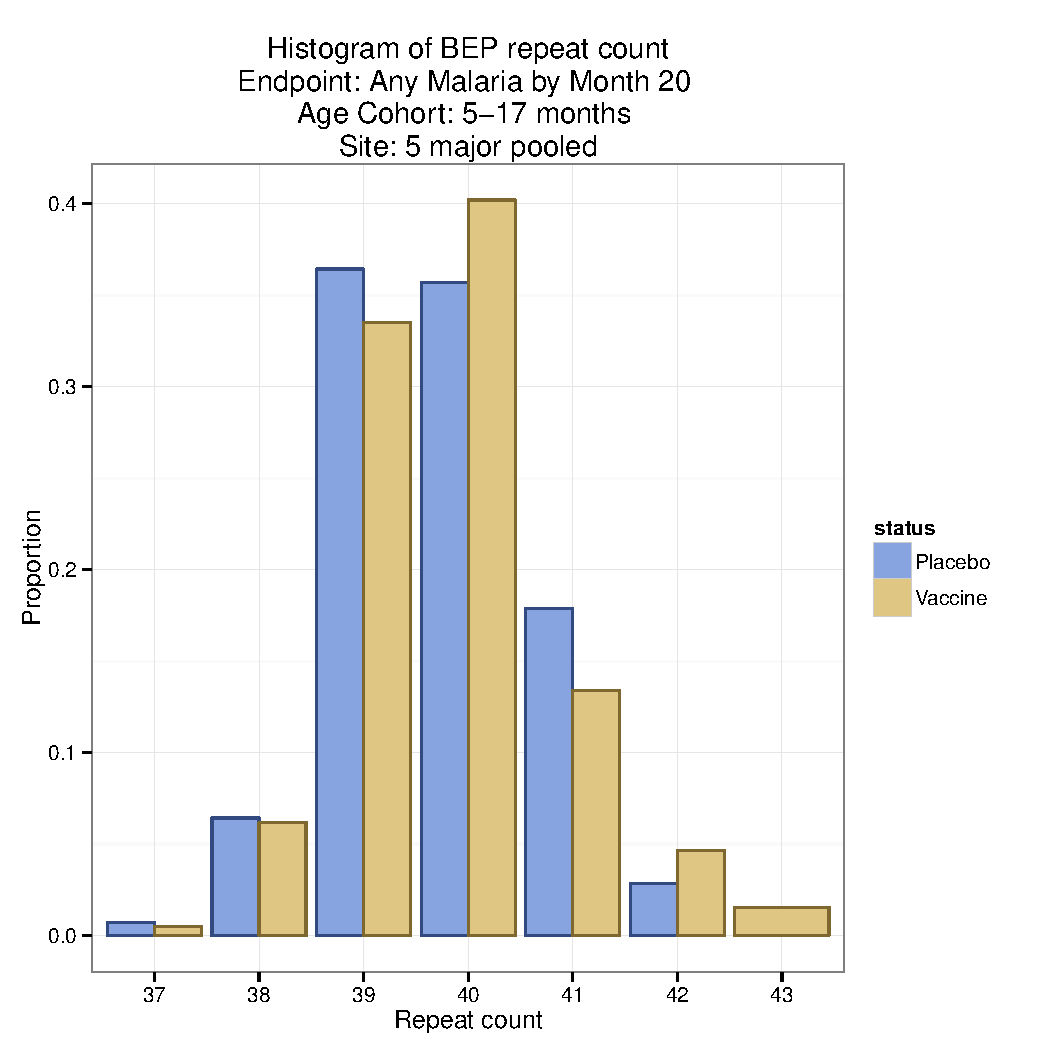
\includegraphics{figures/bep-hist-infant-x-1.pdf}
\caption{Descriptive plot of NANP repeat distribution}
\end{figure}

\subsection{Residue-specific setup}\label{residue-specific-setup}

Load marks file.

Subset to just the 5 major sites.

Collect summary across residues

Plot residue-specific match

\subsection{Residue-specific descriptive
plots}\label{residue-specific-descriptive-plots}

\begin{figure}[htbp]
\centering
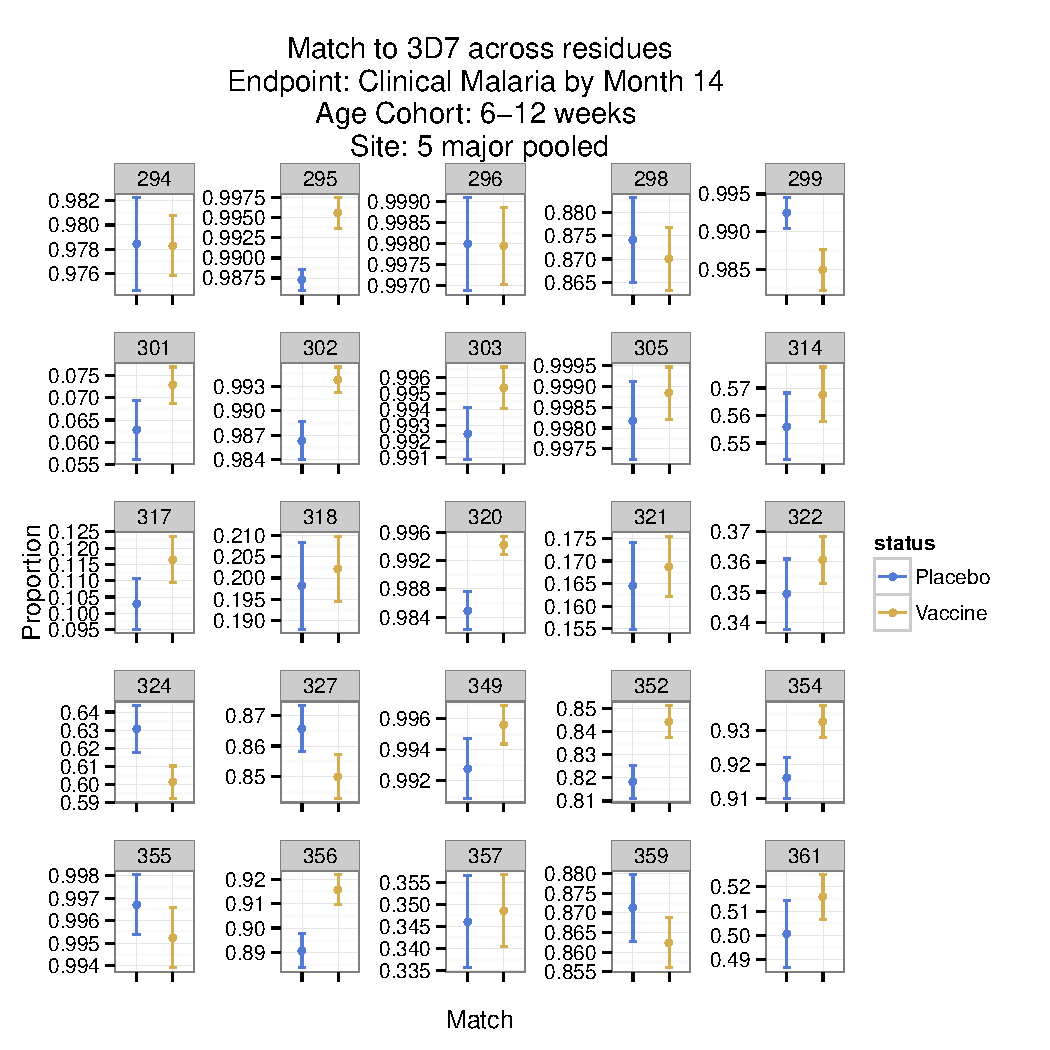
\includegraphics{figures/residue-specific-match-newborn-c-1.pdf}
\caption{Descriptive plot of match to 3D7 in C-terminus CSP}
\end{figure}

\begin{figure}[htbp]
\centering
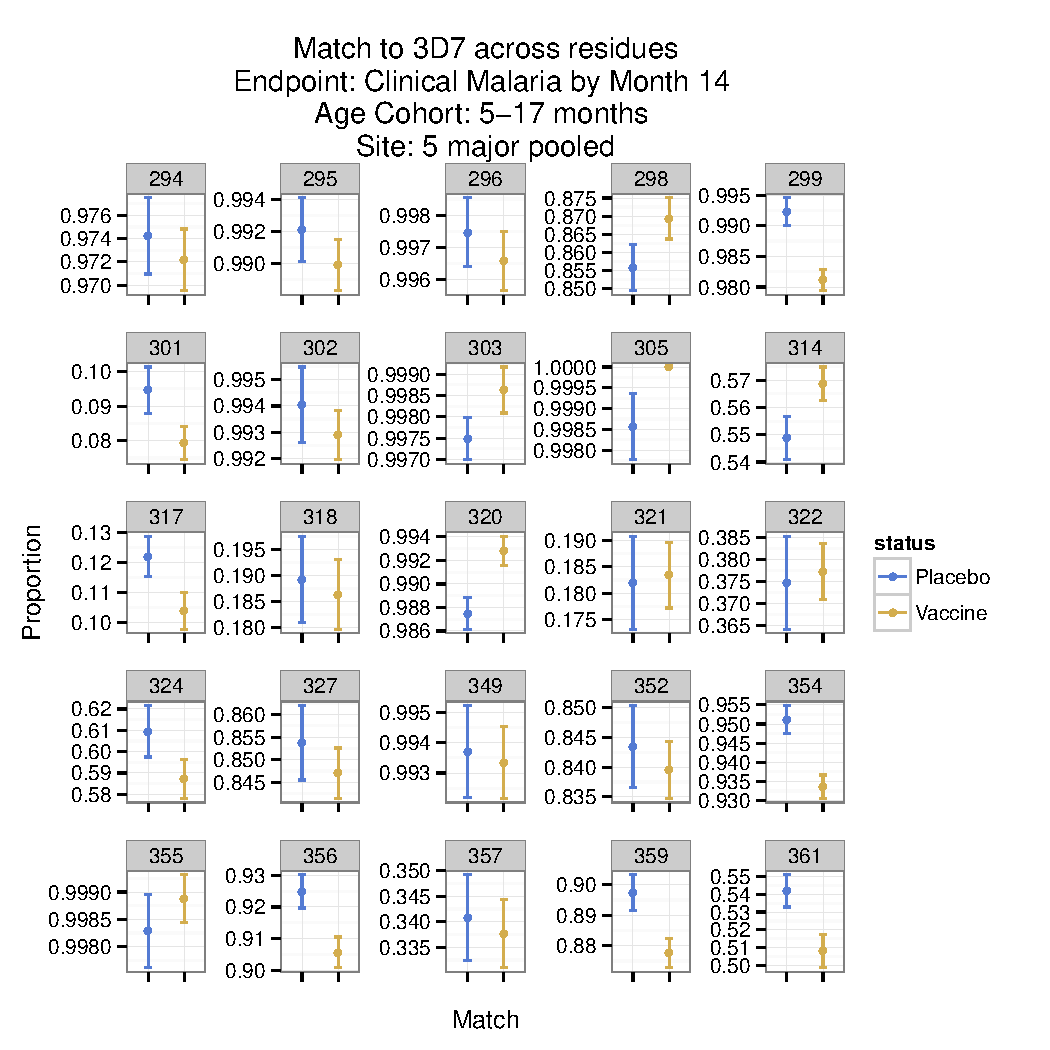
\includegraphics{figures/residue-specific-match-infant-c-1.pdf}
\caption{Descriptive plot of match to 3D7 in C-terminus CSP}
\end{figure}

\begin{figure}[htbp]
\centering
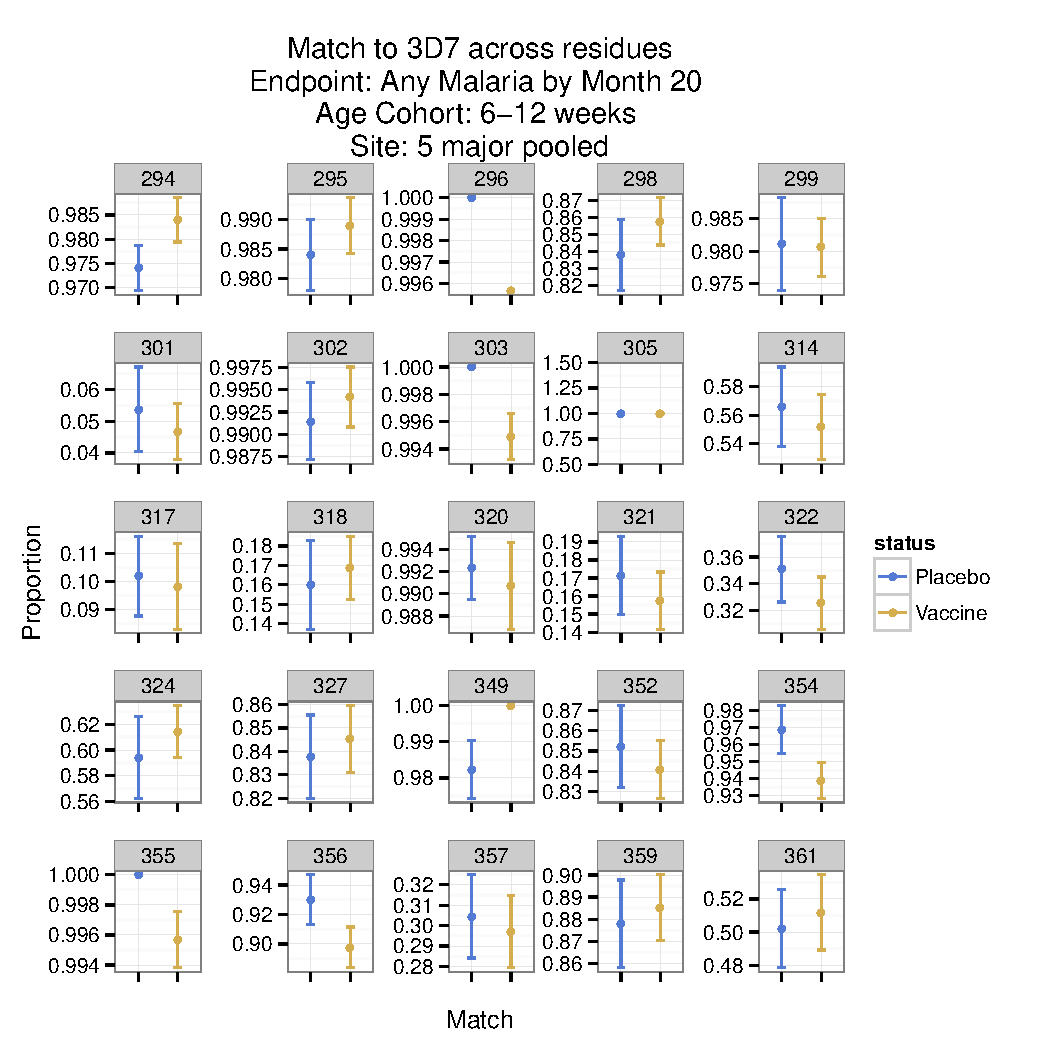
\includegraphics{figures/residue-specific-match-newborn-x-1.pdf}
\caption{Descriptive plot of match to 3D7 in C-terminus CSP}
\end{figure}

\begin{figure}[htbp]
\centering
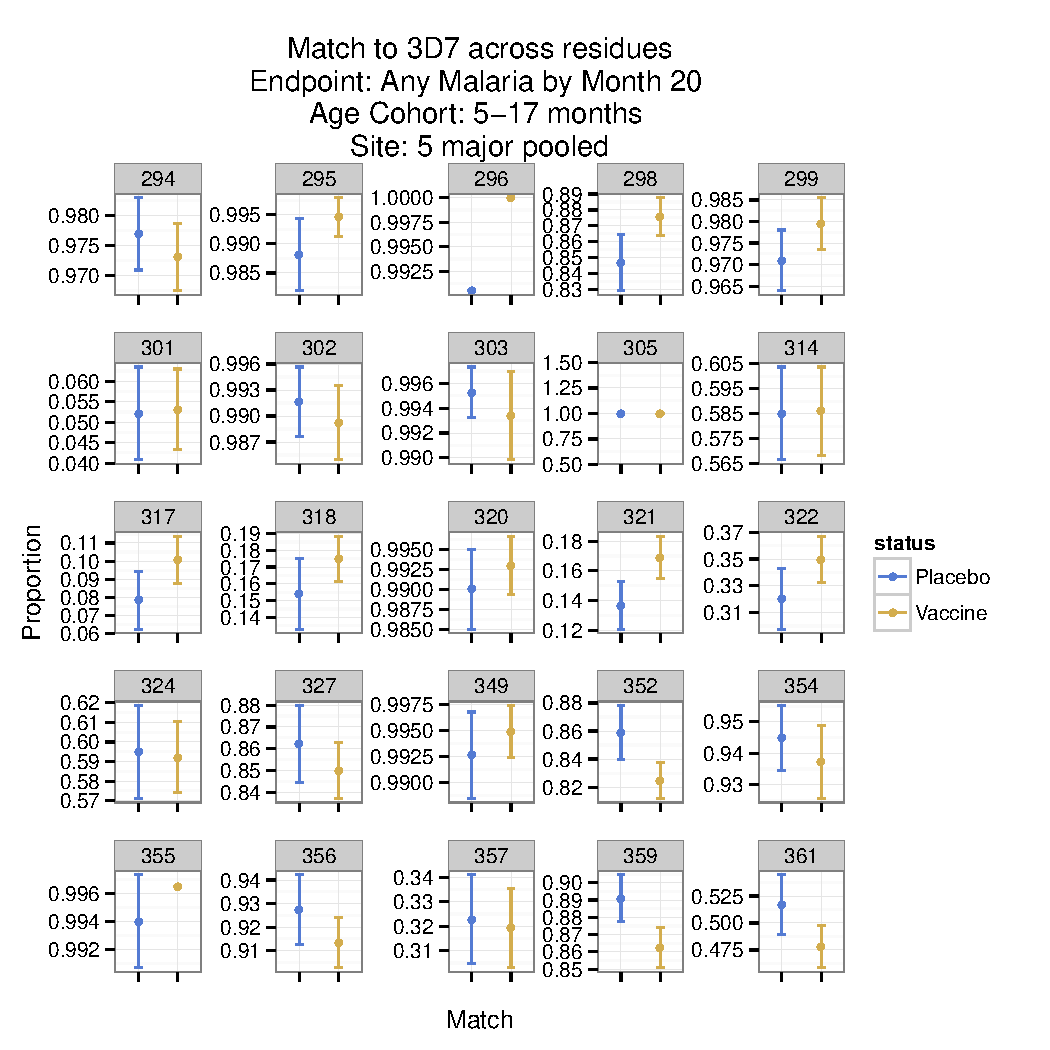
\includegraphics{figures/residue-specific-match-infant-x-1.pdf}
\caption{Descriptive plot of match to 3D7 in C-terminus CSP}
\end{figure}

\end{document}
